\documentclass[UTF8,a4paper]{paper}
\usepackage[utf8]{inputenc}
\usepackage{ctex}
\usepackage{amsmath}
\usepackage{pdfpages}
\usepackage{graphicx}
\usepackage{wrapfig}
\usepackage{listings}
\usepackage{multicol}
\usepackage{float}
\usepackage{appendix}
\title{第三次仿真实验报告}
\author{张蔚桐\ 2015011493\ 自55}
\begin {document}
\newcommand{\tabincell}[2]{\begin{tabular}{@{}#1@{}}#2\end{tabular}}
\maketitle
\tableofcontents
\clearpage
\section{一阶微分方程求解电路}
\subsection{电路 }
我们使用一节运放搭建一节微分求解电路求解方程
\begin{equation}
u_I=a * u_O+b*\frac{\mathrm{d}u_O}{\mathrm{d}t}
\label{eq1}
\end{equation}
我们考虑整个电路中出现了微分,如果直接实现这个电路,涉及到微分器,但是由于微分器容易受到电路中噪声的干扰,因此实际电路中经常使用积分代替微分实现电路,因此我们将方程\ref{eq1}的两侧积分得到:
\begin{equation}
\int_0^tu_i\mathrm{d}t =a\int_0^tu_o\mathrm{d}t + b u_O
\label{eq2}
\end{equation}
这里我们假定了电路的初始条件为0,即$u_O(0)=0,\displaystyle{\frac{\mathrm{d}u_O}{\mathrm{d}t}(0)=0}$ 
因此我们可以根据式\ref{eq2}整理成运放的工作方程
\begin{equation}
u_o=\frac{1}{b}\int_0^tu_I-au_O\mathrm{d}t
\label{eq3}
\end{equation}
这提示我们电路是一个积分——减法器,因此我们设计图\ref{cir1}的电路实现相关的电路。其中两个电阻$R_a,R_b$(图中表示为a和b)的阻值分别由方程参数确定,分别为
$$\begin{cases}
R_a= 10\mathrm{k}\Omega \times a\\
R_b=10\mathrm{k}\Omega \times b
\end{cases}$$
在这种情况下,运放$U_1$输出的电压为所求的电压$u_O$,因此我们可以得到运放$U_3$输出的电压是$-au_O$,进一步得到运放$U_2$输出的电压是
$$\int_0^t(u_I-au_O)\mathrm{d}t$$
于是利用运放$U_1$可以得到方程

\begin{equation}
u_O=\frac{1}{b}\int_0^t(u_I-au_O)\mathrm{d}t
\label{eq4}
\end{equation}
可以看出式子\ref{eq4}和\ref{eq3}相同,电路实现了要求
\begin{figure}
\centering
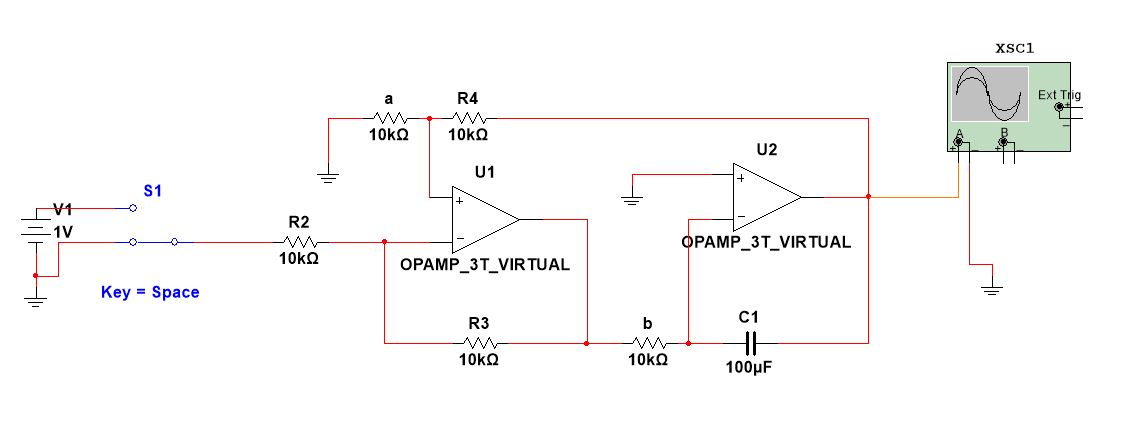
\includegraphics[width=\textwidth]{cir1.jpg}
\caption{求解一阶微分方程的运算电路}
\label{cir1}
\end{figure}
\subsection{具体情况的求解}
尝试带入一些参数来解方程验证电路的特性,我们采用阶跃输入来验证电路特性

\begin{multicols}{2}
\begin{figure}[H]
\centering
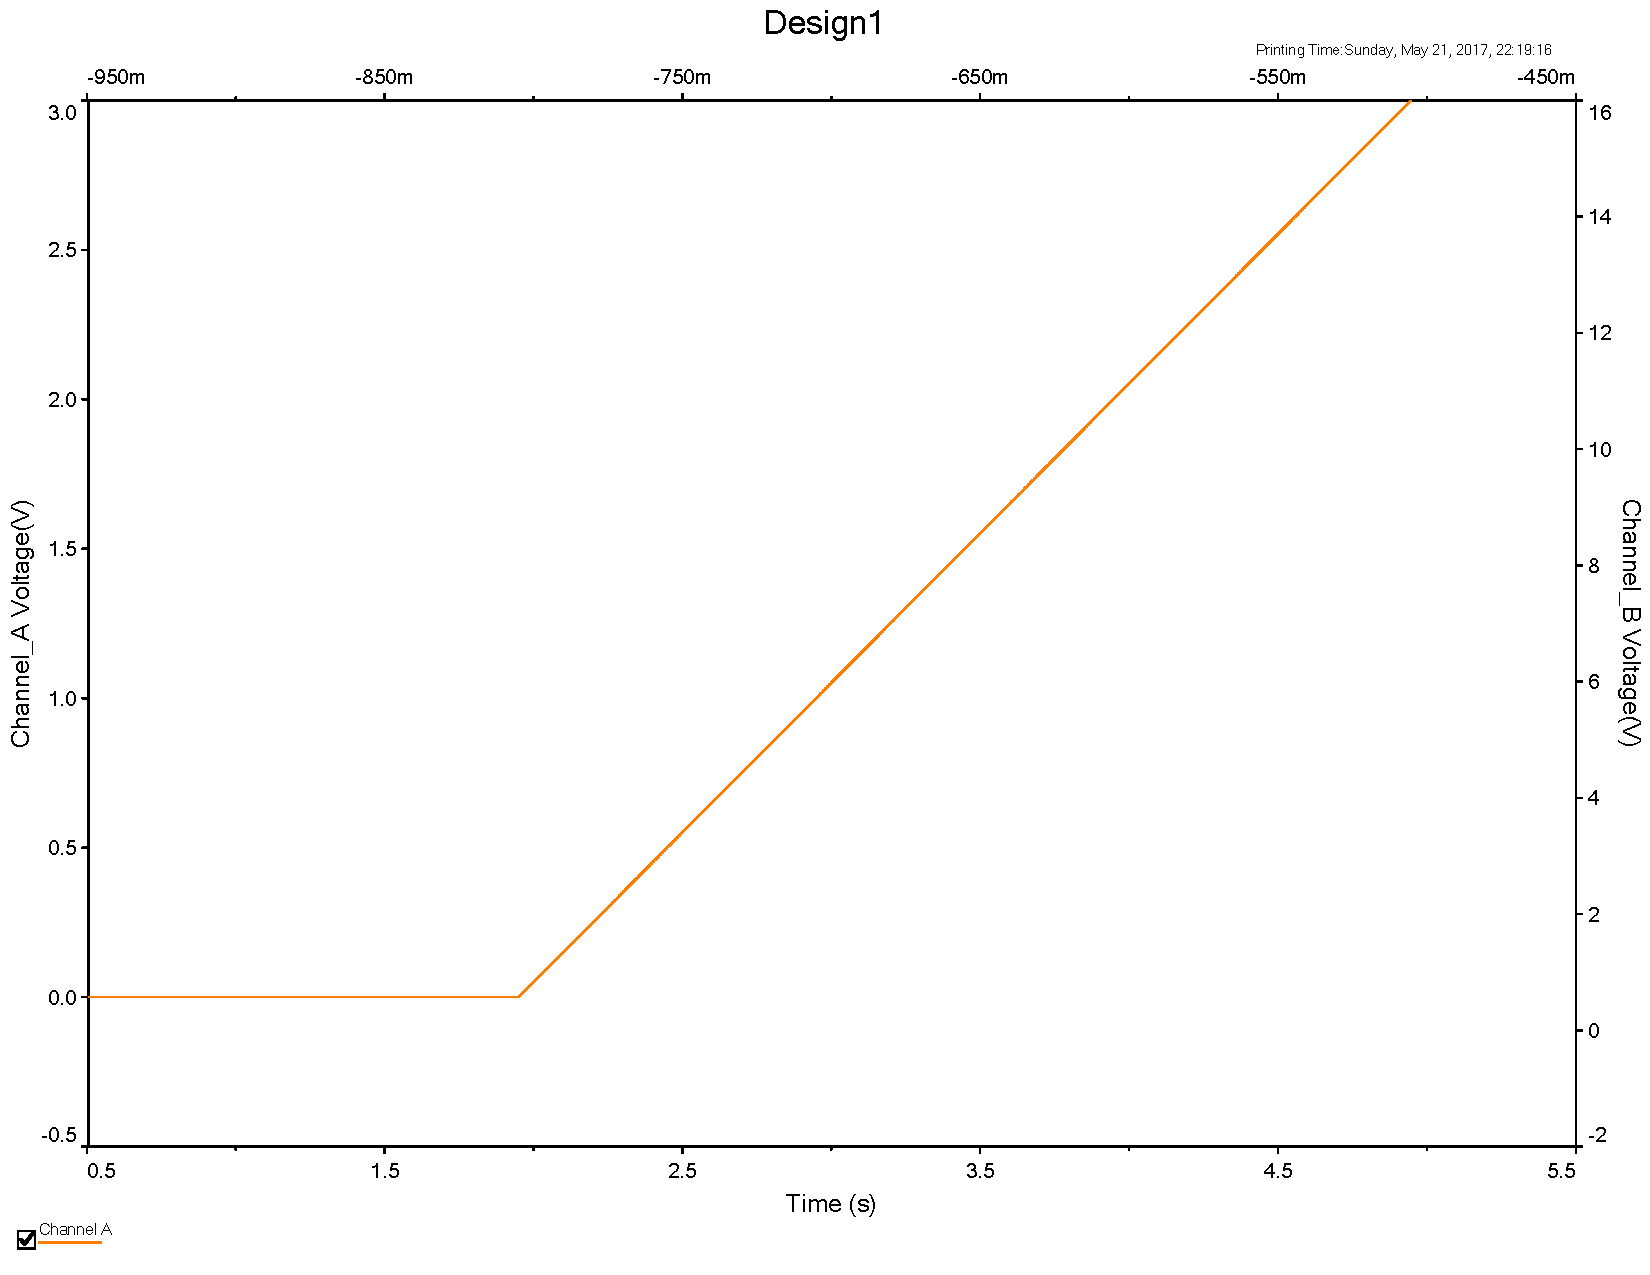
\includegraphics[width=\columnwidth]{a0b1.pdf}
\caption{$a=0,b=1$时的情况}
\label{a0b1}
\end{figure}
\begin{figure}[H]
\centering
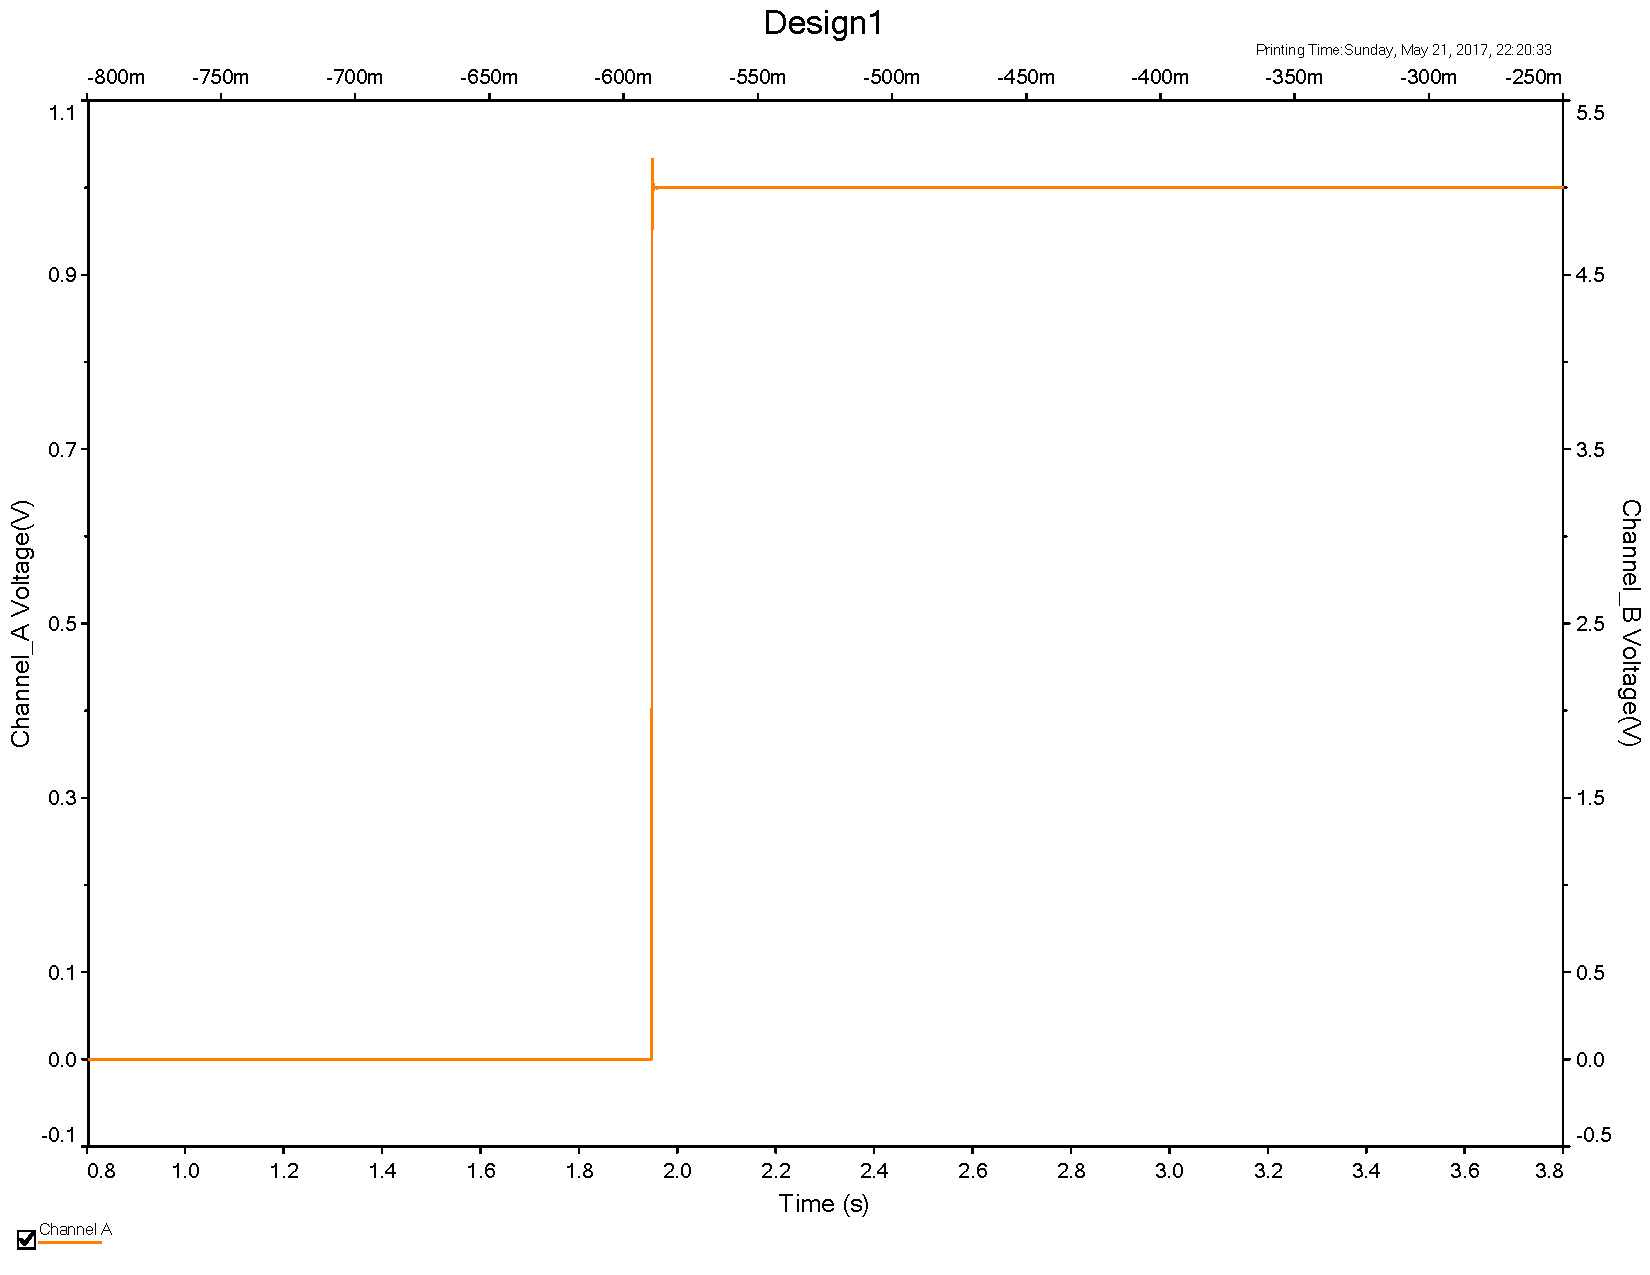
\includegraphics[width=\columnwidth]{a1b0.pdf}
\caption{$a=1,b=0$时的情况}
\label{a1b0}
\end{figure}	
\begin{figure}[H]
\centering
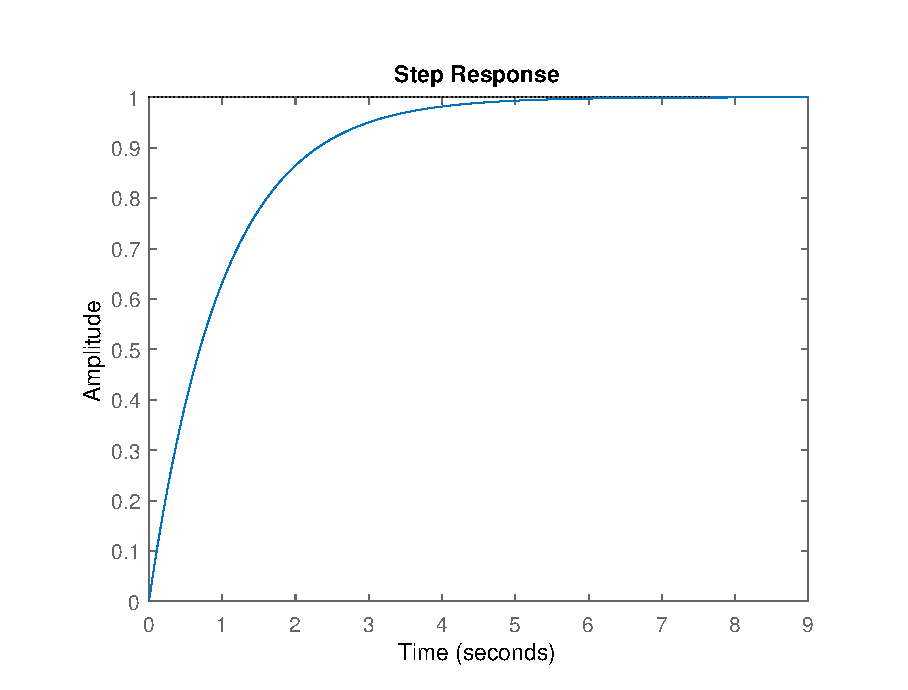
\includegraphics[width=\columnwidth]{the.eps}
\caption{$a=1,b=1$时的理论分析情况}
\label{the}
\end{figure}
\begin{figure}[H]
\centering
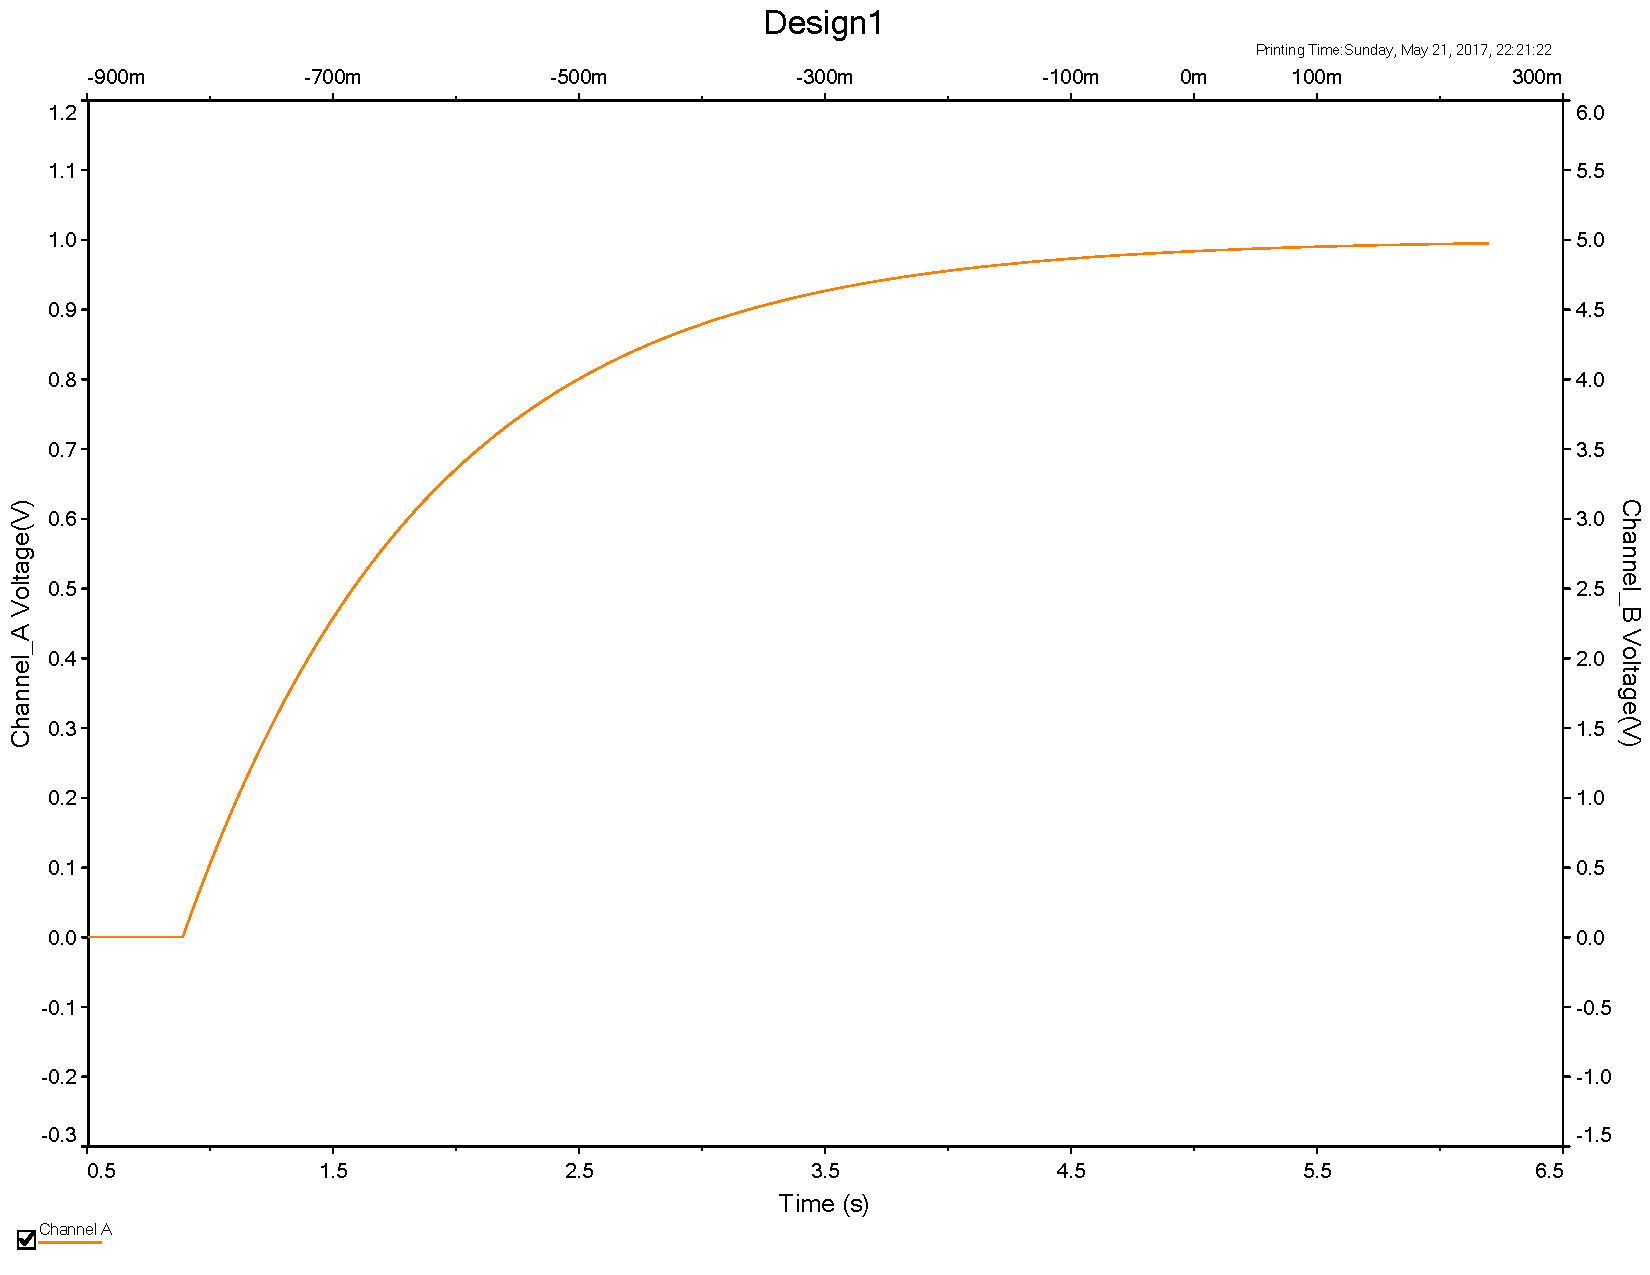
\includegraphics[width=\columnwidth]{a1b1.pdf}
\caption{$a=1,b=1$时的情况}
\label{a1b1}
\end{figure}
\end{multicols}

$a=0,b=1$:此时方程退化为$u_I=\frac{\mathrm{d}u_O}{\mathrm{d}t}$输出电压是输入电压的积分,如图\ref{a0b1}所示,在电压没有超过运放摆幅时是一个线性增加的电路,并且可以看出斜率基本为1V/s

$a=1,b=0$:此时方程退化为$u_I=u_O$输出电压是输入电压的跟随,如图\ref{a1b0}所示,输出电压的确是输入电压的一个跟随

$a=1,b=1$:此时方程为$u_I=u_O+\frac{\mathrm{d}u_O}{\mathrm{d}t}$因此得到电路的传递函数为
$G(s)=\frac{1}{s+1}$,利用MATLAB中的相关函数可以求得阶跃响应如图\ref{the}所示,从图\ref{a1b1}中可以看出和理论计算差距不大。

从上面几个实例中可以看出电路工作特性良好
\section{VCVS电路搭建和测试}
\subsection{辐频相频特性的测量}
\subsubsection{VCVS低通滤波电路搭建和测试}
\begin{figure}[h]
\centering
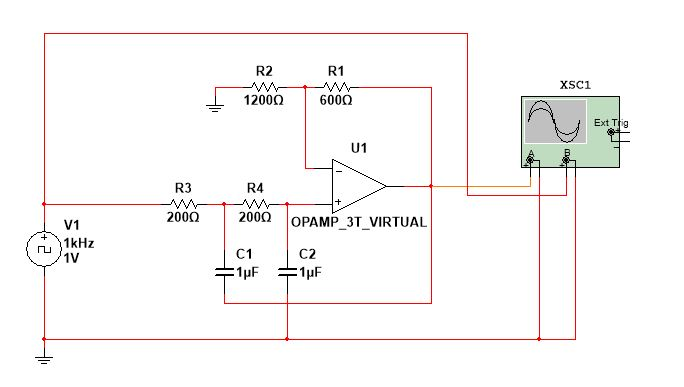
\includegraphics[width=\textwidth]{L.jpg}
\caption{VCVS低通滤波电路}
\label{L}
\end{figure}

采用经典的VCVS设计,我们可以得到如图\ref{L}的低通滤波电路,并且可以得到特征频率$f_0=\frac{1}{2\pi RC}$,在VCVS电路中,$f_0\approx f_P$,可以近似作为相关电路参数的选择条件,而如果想得到更准确的电路参数,可能需要进一步的调参。

我们可以看出,如图\ref{LQ1},\ref{LQ23},\ref{LQ10}所示,随着电路$Q$值的增大,在转折点附近的反冲增大,甚至出现明显的共振峰。同时$Q$的增大在一定程度上也使得$f_P$更加接近$f_0$,在这一点上也提升了电路的特性。.

可以看到,低通滤波器的相频曲线从0逐渐变为-180,随着Q值的增大,相变的位置逐渐收敛到特征频率$f_0$的位置,使得相频特性更加趋近于一个阶跃函数的形式。
\begin{multicols}{3}
\begin{figure}[H]
\centering
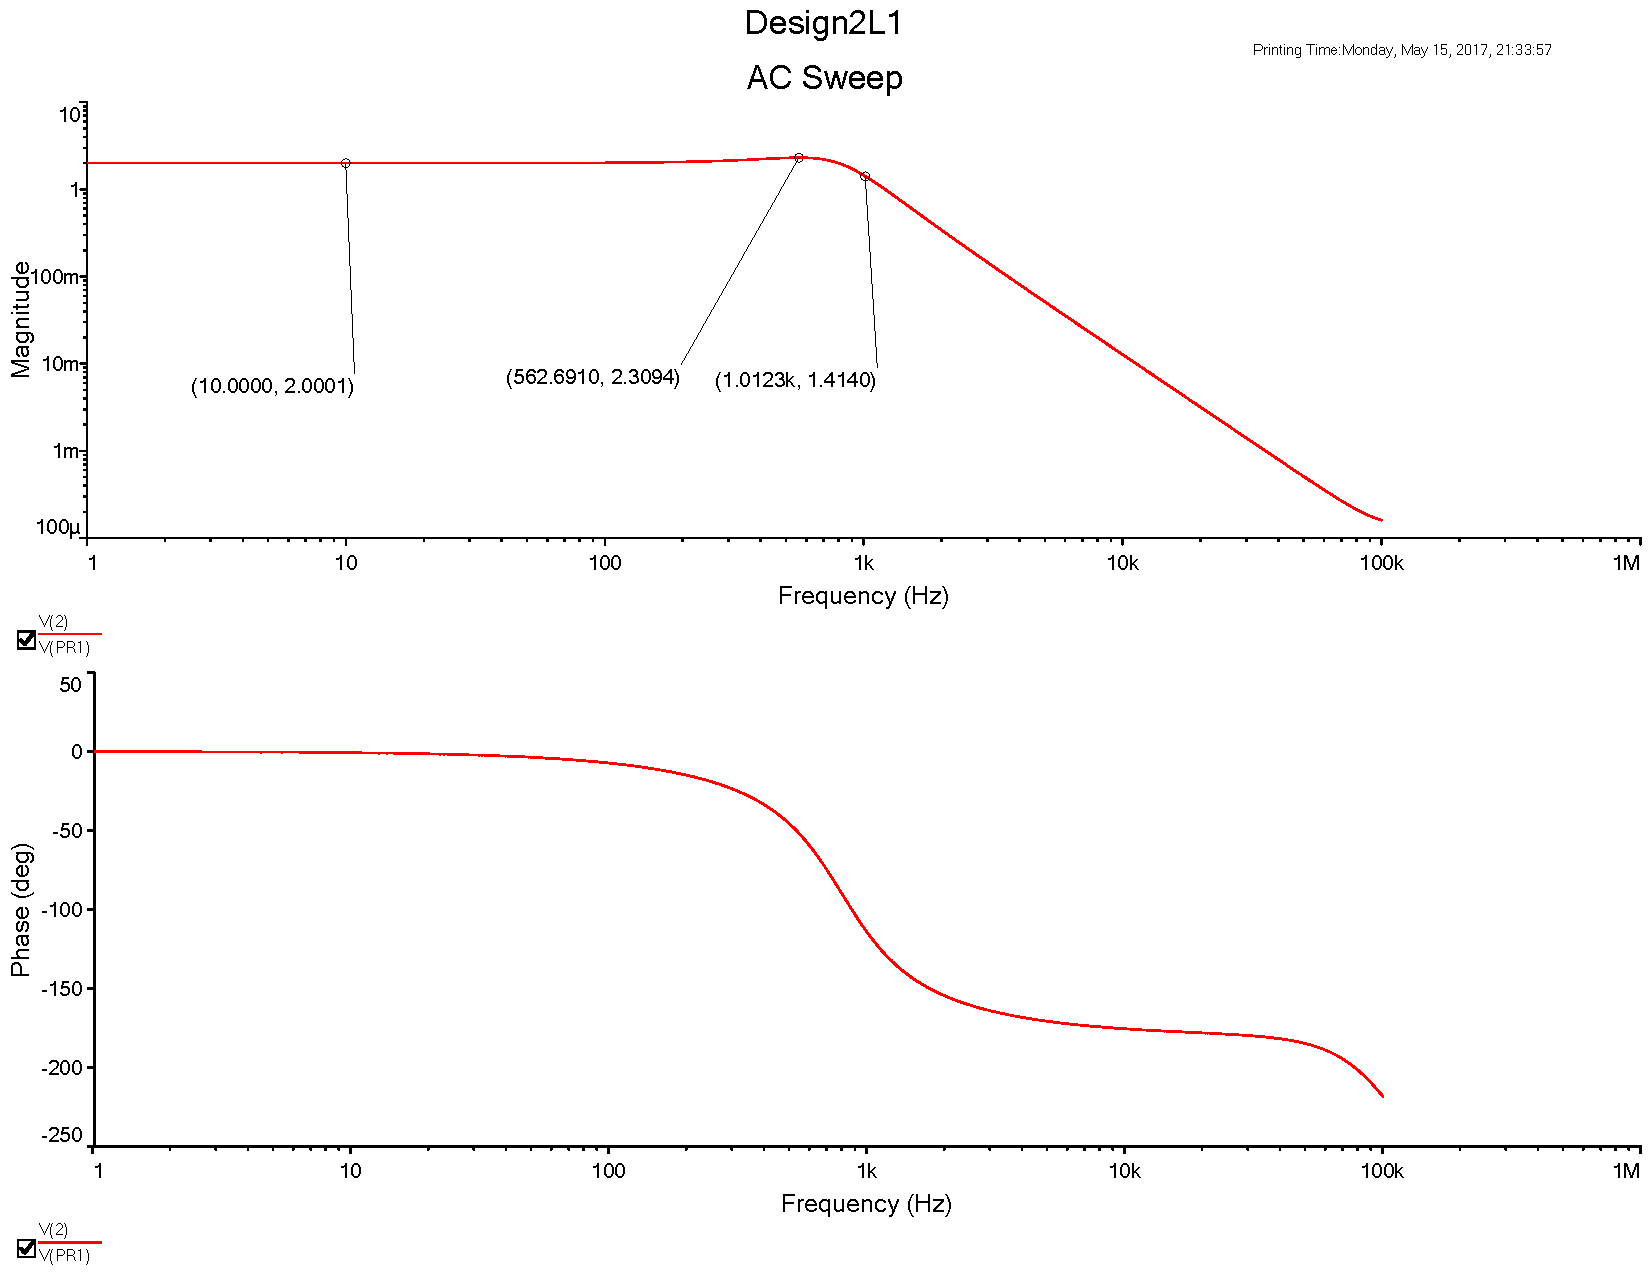
\includegraphics[width=\columnwidth]{2L1.pdf}
\caption{$Q=1$}
\label{LQ1}
\end{figure}
\begin{figure}[H]
\centering
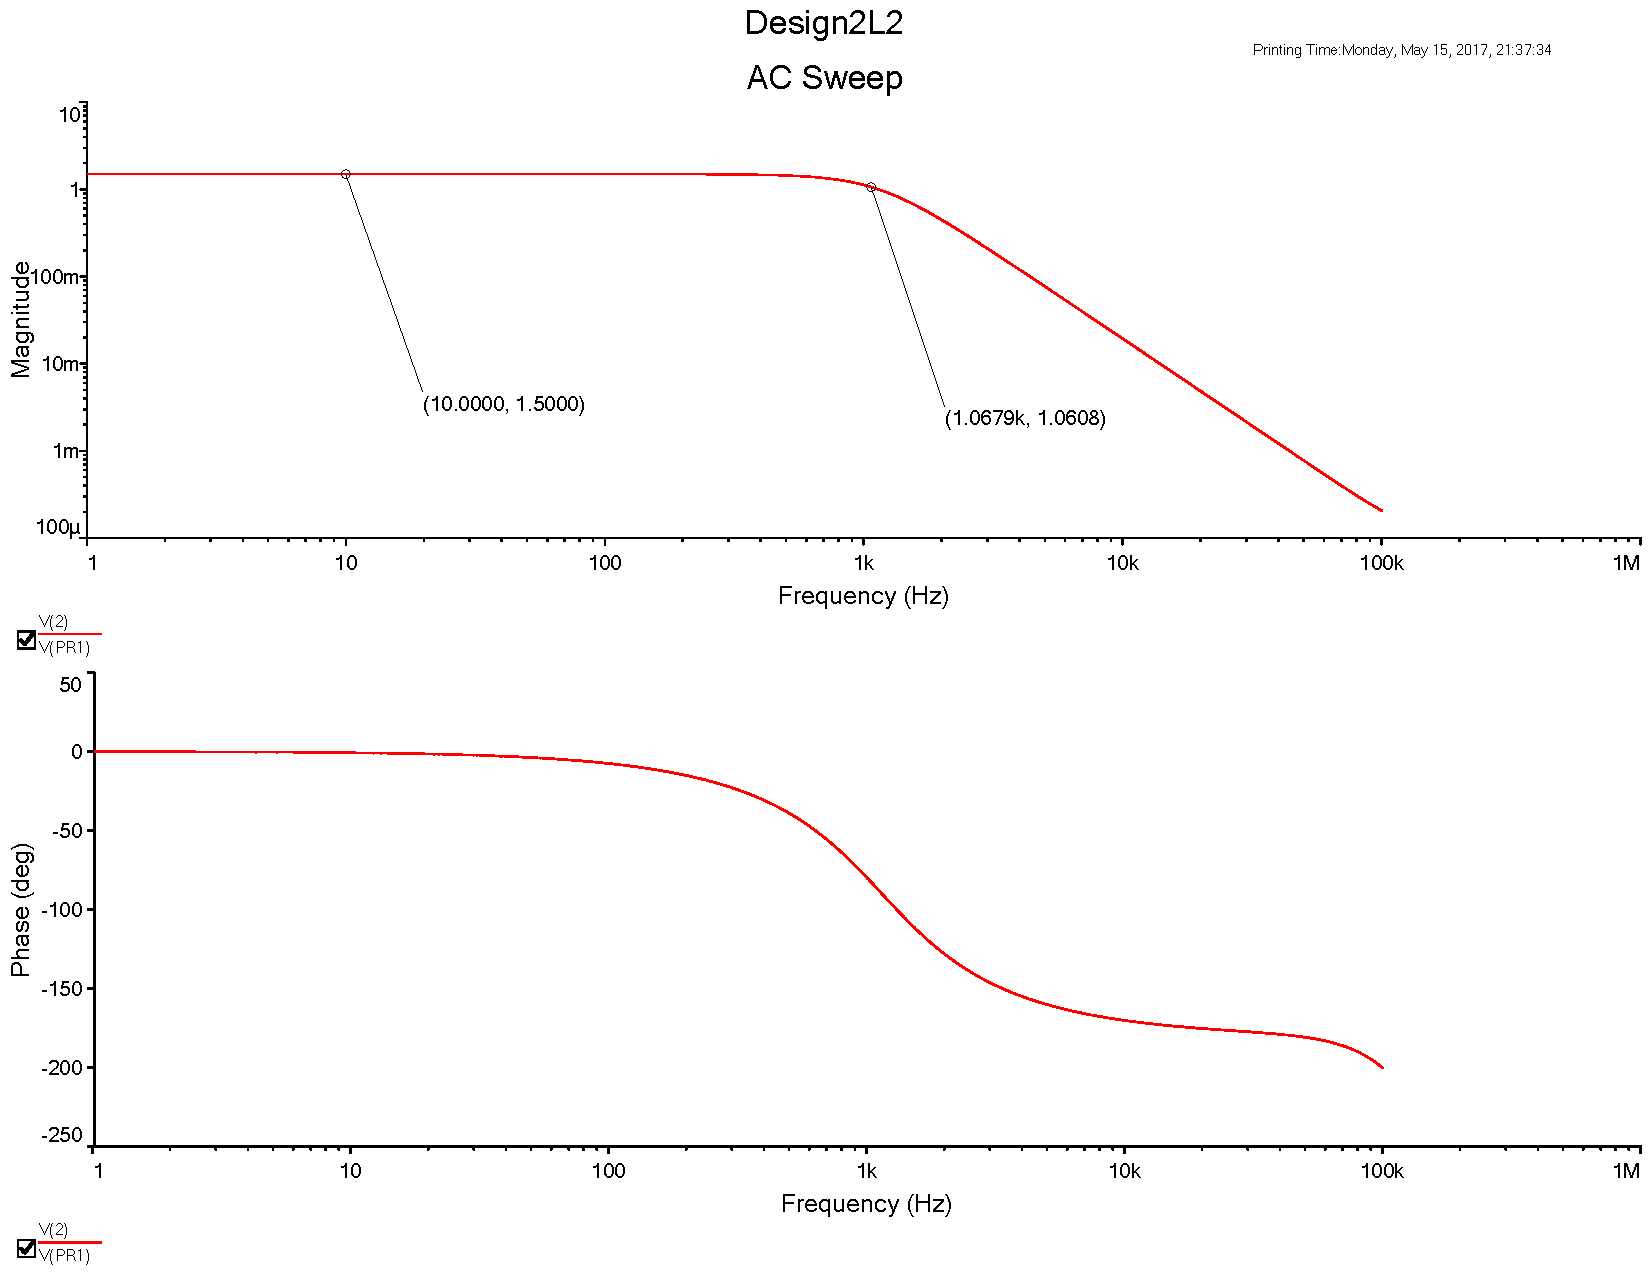
\includegraphics[width=\columnwidth]{2L2_3.pdf}
\caption{$Q=2/3$}
\label{LQ23}
\end{figure}
\begin{figure}[H]
\centering
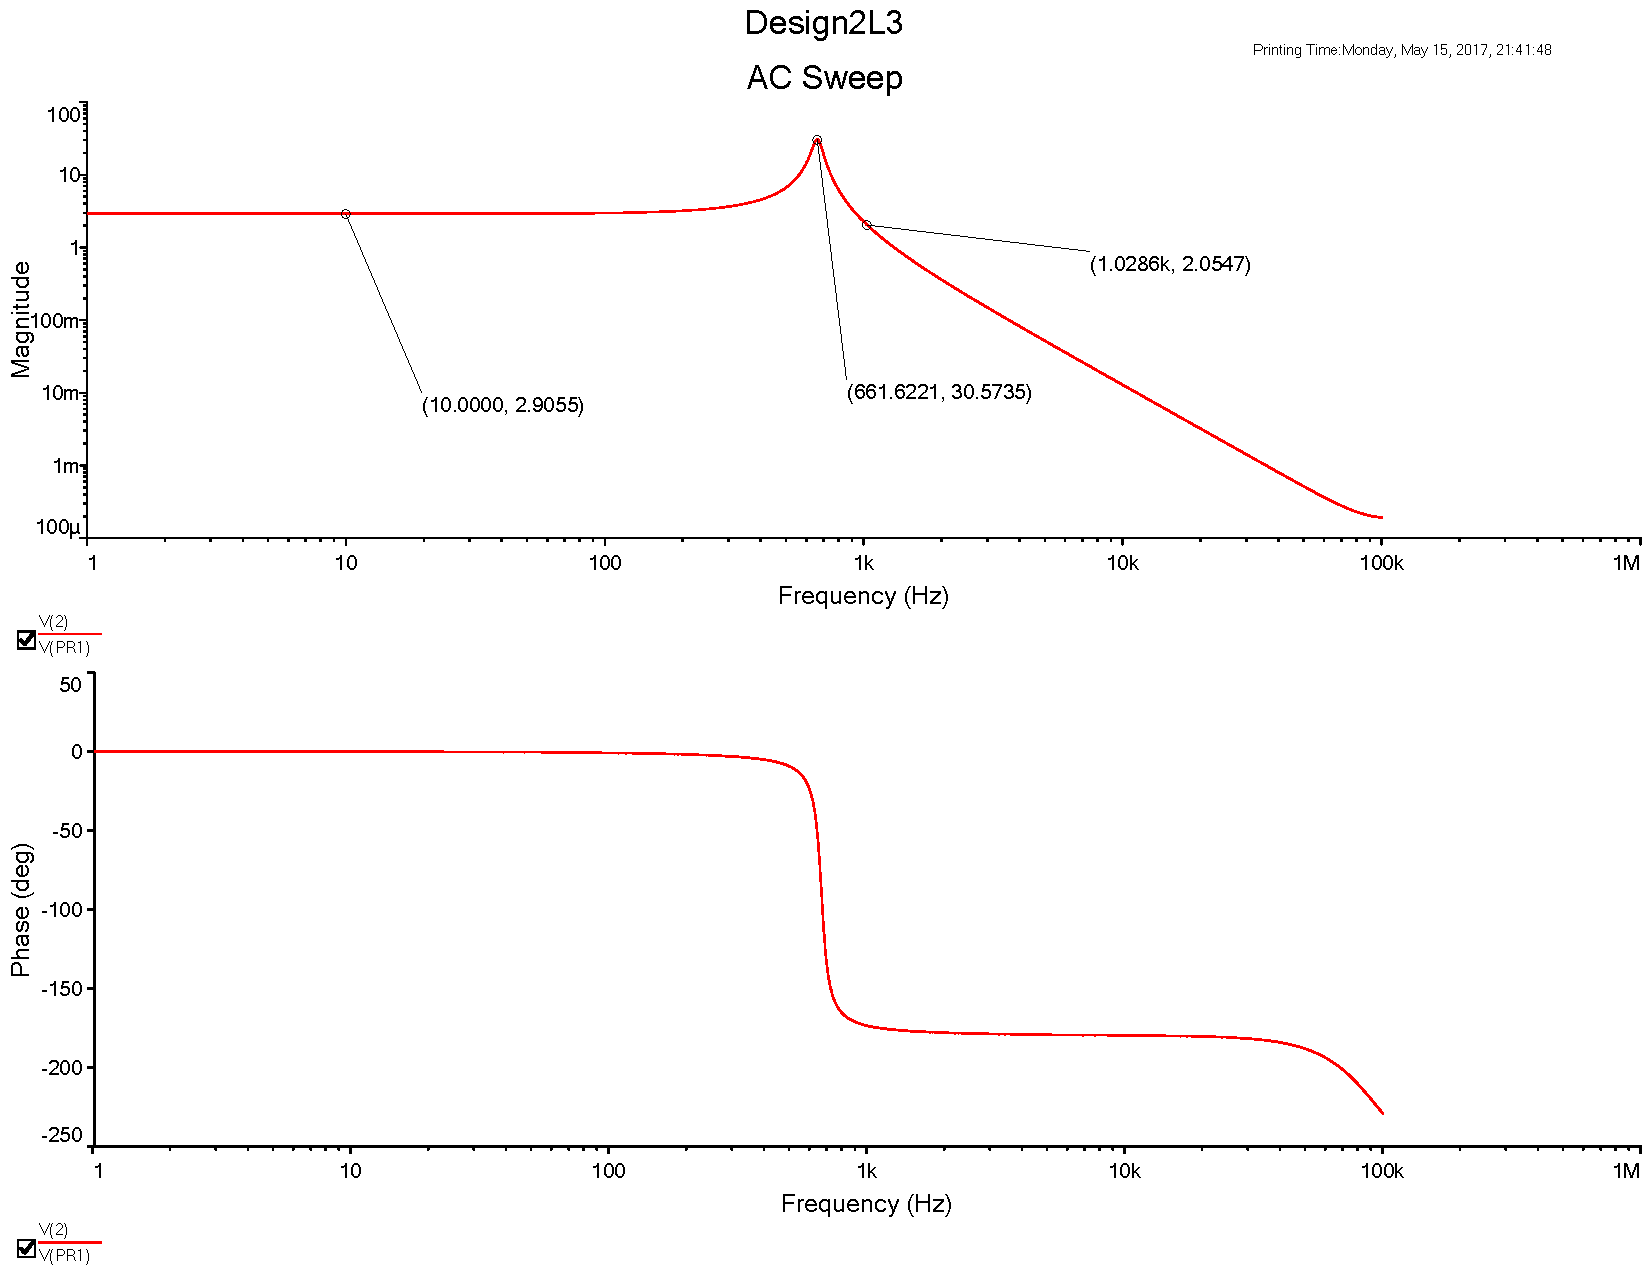
\includegraphics[width=\columnwidth]{2L10_5.pdf}
\caption{$Q=10.5$}
\label{LQ10}
\end{figure}
\end{multicols}
\subsubsection{VCVS高通滤波电路搭建和测试}
\begin{figure}
\centering
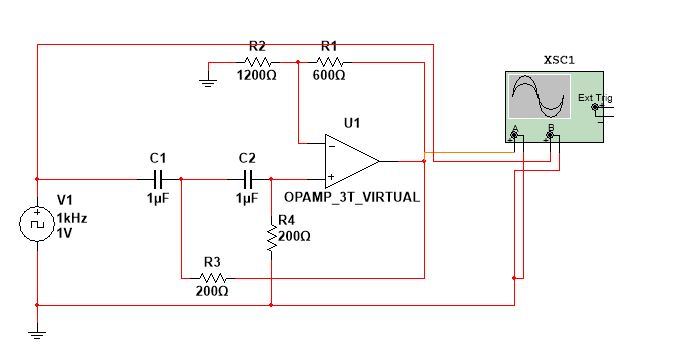
\includegraphics[width=\textwidth]{H.jpg}
\caption{VCVS高通滤波电路}[h]
\label{H}
\end{figure}
采用经典的VCVS设计,我们可以得到如图\ref{H}的高通滤波电路,并且可以得到特征频率$f_0=\frac{1}{2\pi RC}$,在VCVS电路中,$f_0\approx f_P$,可以近似作为相关电路参数的选择条件,而如果想得到更准确的电路参数,可能需要进一步的调参。

\begin{multicols}{3}
\begin{figure}[H]
\centering
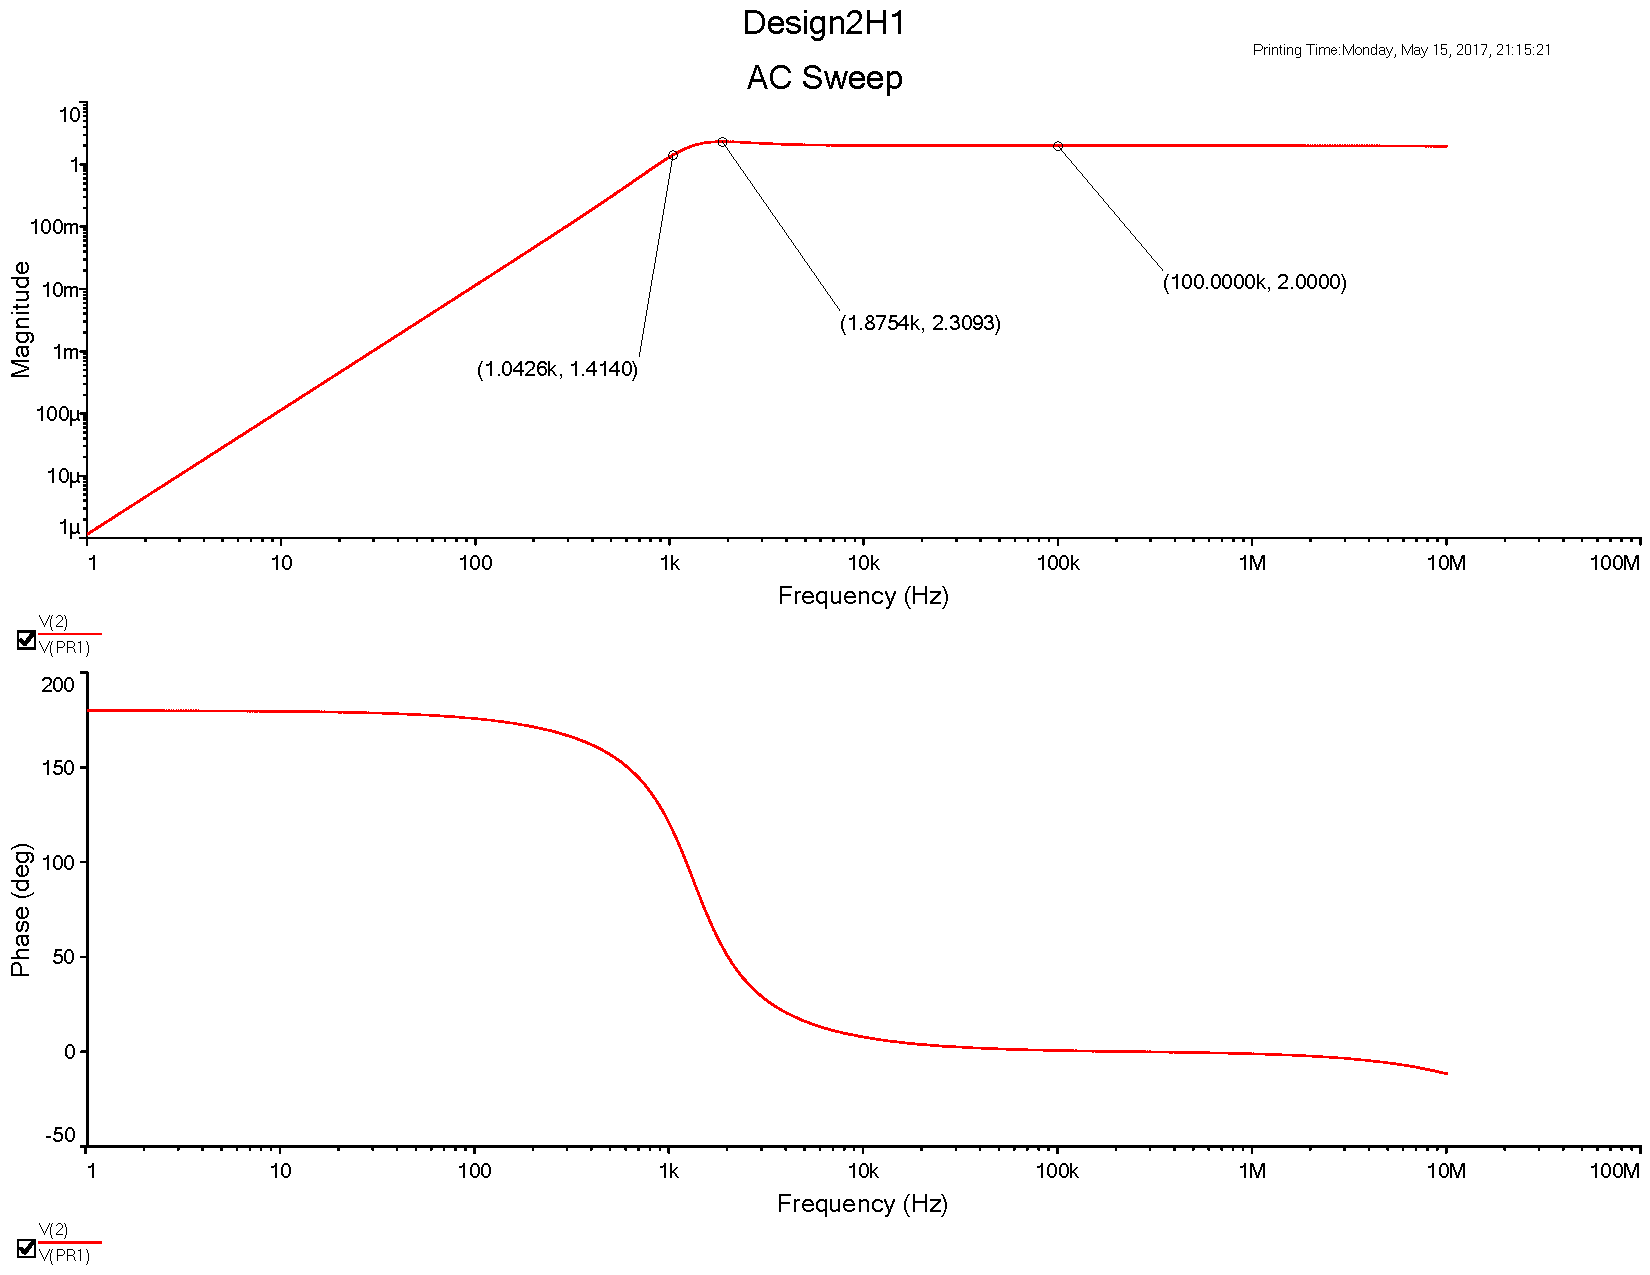
\includegraphics[width=\columnwidth]{2H1.pdf}
\caption{$Q=1$}
\label{HQ1}
\end{figure}
\begin{figure}[H]
\centering
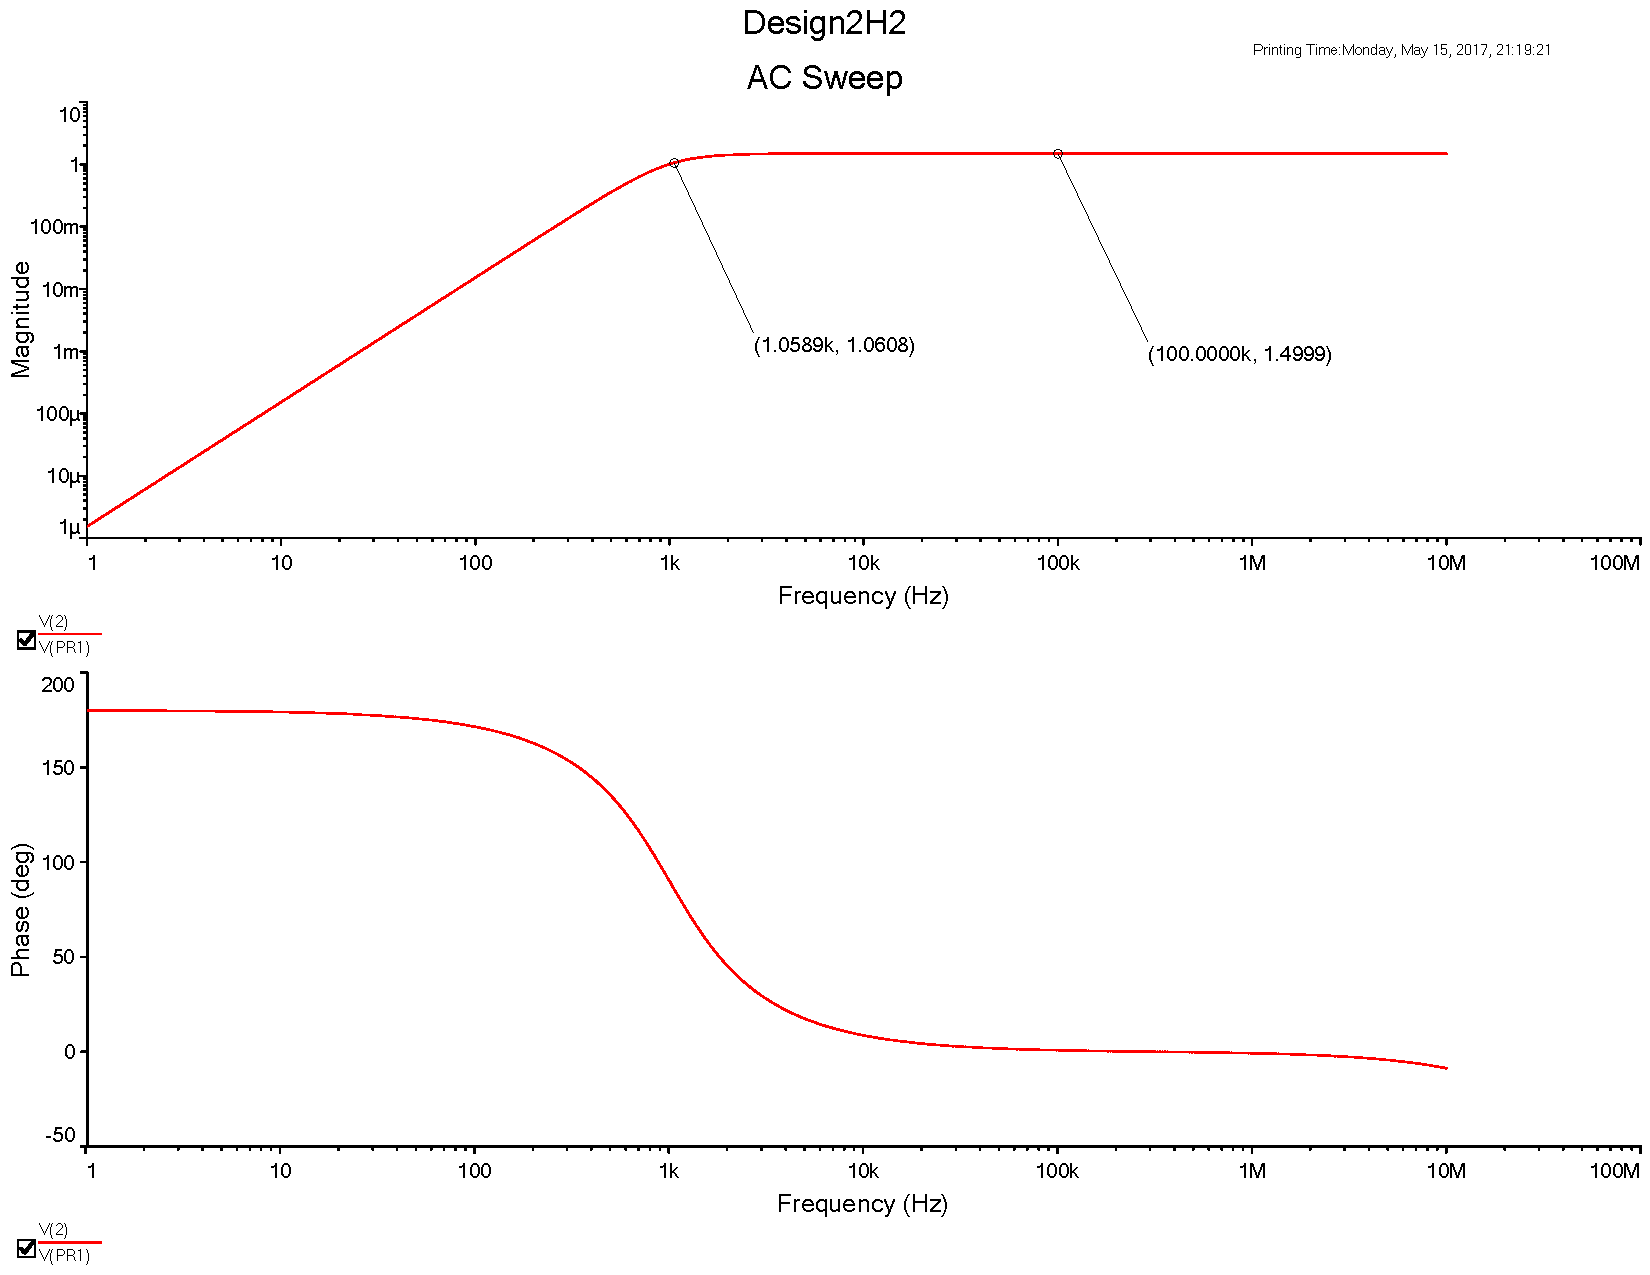
\includegraphics[width=\columnwidth]{2H2_3.pdf}
\caption{$Q=2/3$}
\label{HQ23}
\end{figure}
\begin{figure}[H]
\centering
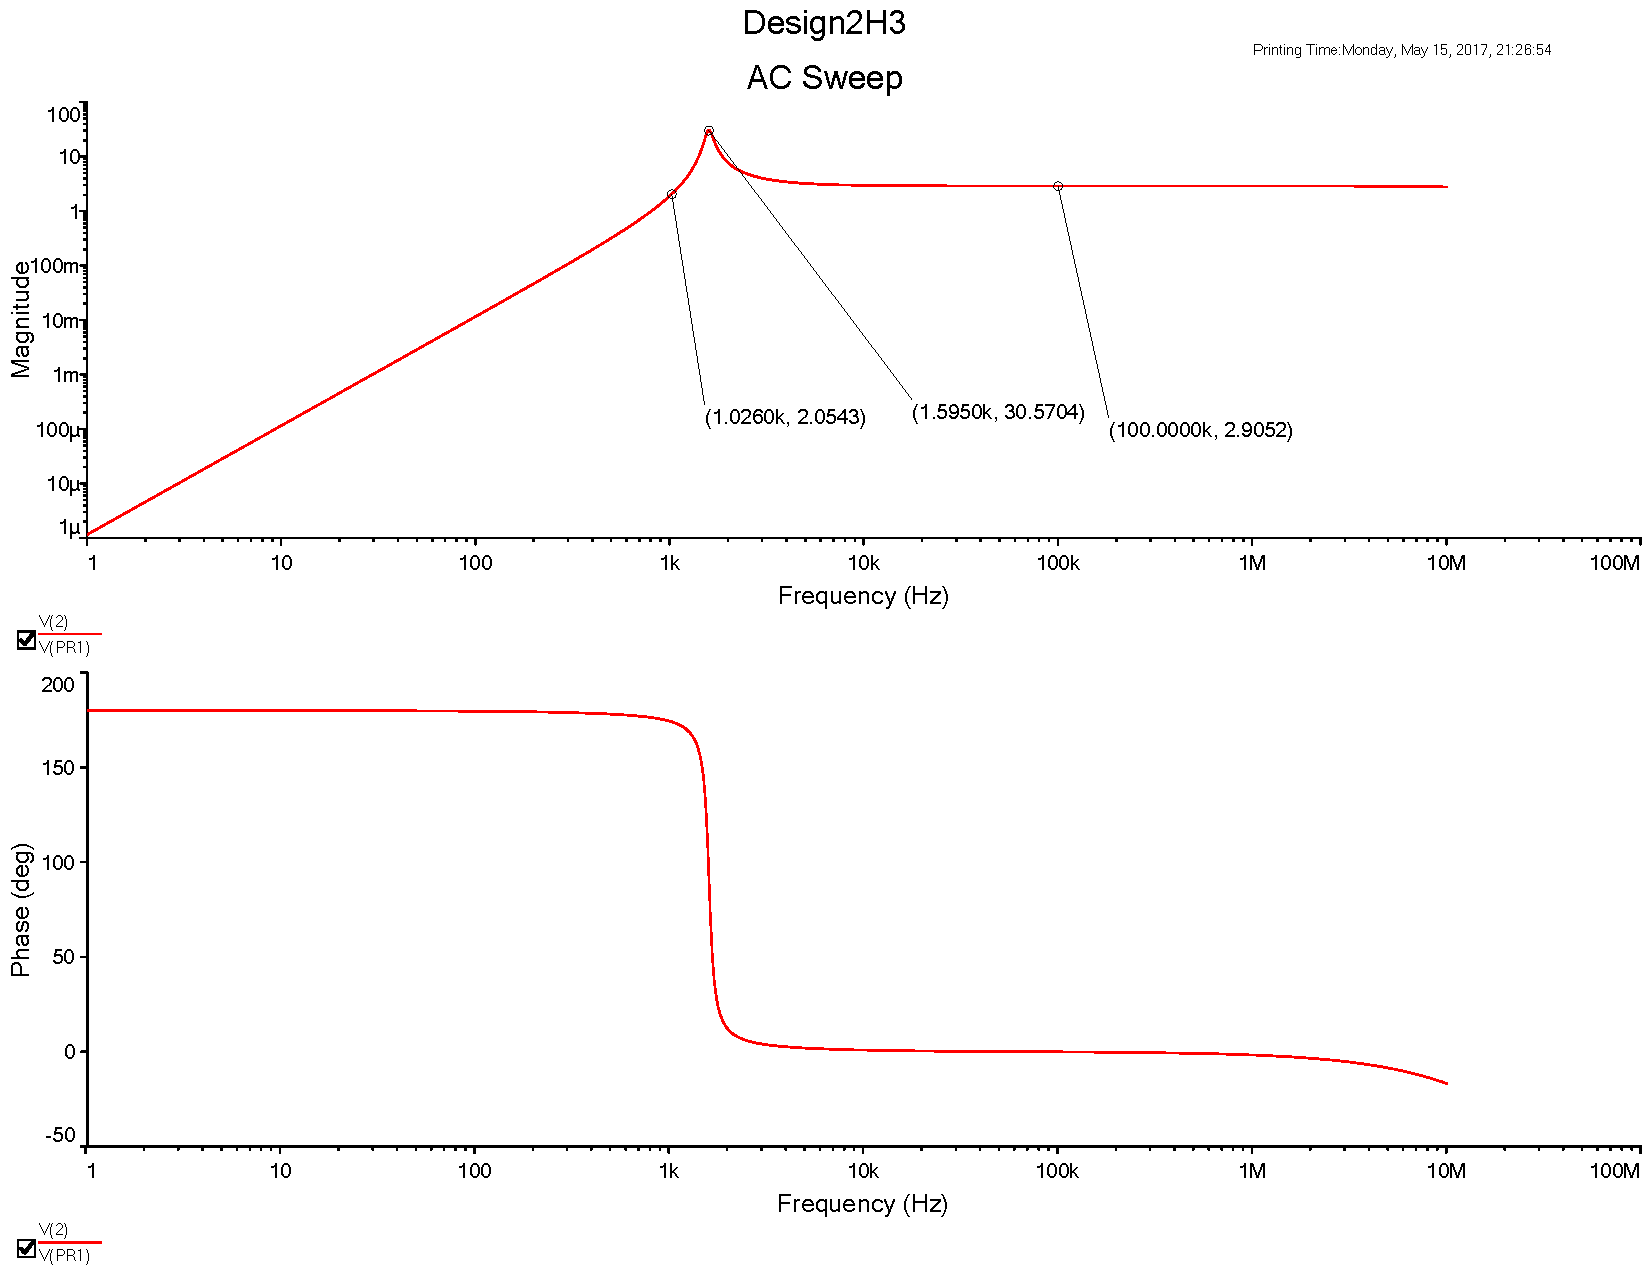
\includegraphics[width=\columnwidth]{2H10_5.pdf}
\caption{$Q=10.5$}
\label{HQ10}
\end{figure}
\end{multicols}

我们可以看出,如图\ref{HQ1},\ref{HQ23},\ref{HQ10}所示,随着电路$Q$值的增大,在转折点附近的反冲增大,甚至出现明显的共振峰。同时$Q$的增大在一定程度上也使得$f_P$更加接近$f_0$,在这一点上也提升了电路的特性。

可以看到,低通滤波器的相频曲线从180逐渐变为0,随着Q值的增大,相变的位置逐渐收敛到特征频率$f_0$的位置,使得相频特性更加趋近于一个阶跃函数的形式。
\subsubsection{VCVS带通滤波电路搭建和测试}
\begin{figure}[h]
\centering
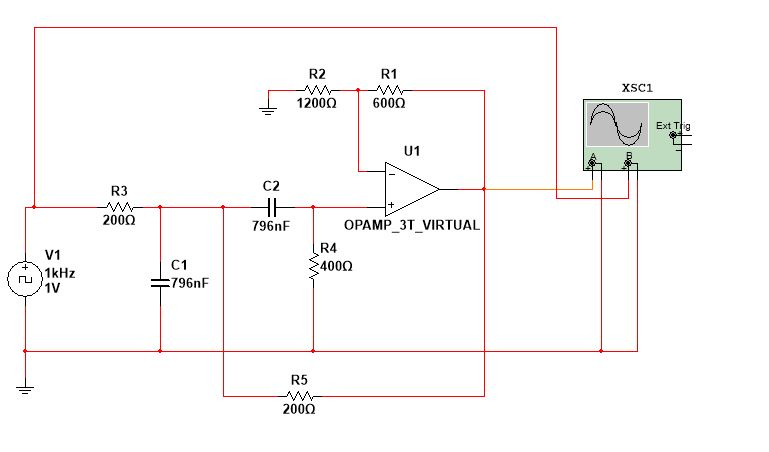
\includegraphics[width=\columnwidth]{P.jpg}
\caption{VCVS带通滤波电路}
\label{P}
\end{figure}
采用经典的VCVS设计,我们可以得到如图\ref{H}的带通滤波电路,并且可以得到特征频率$f_0=\frac{1}{2\pi RC}$。

\begin{multicols}{2}
\begin{figure}[H]
\centering
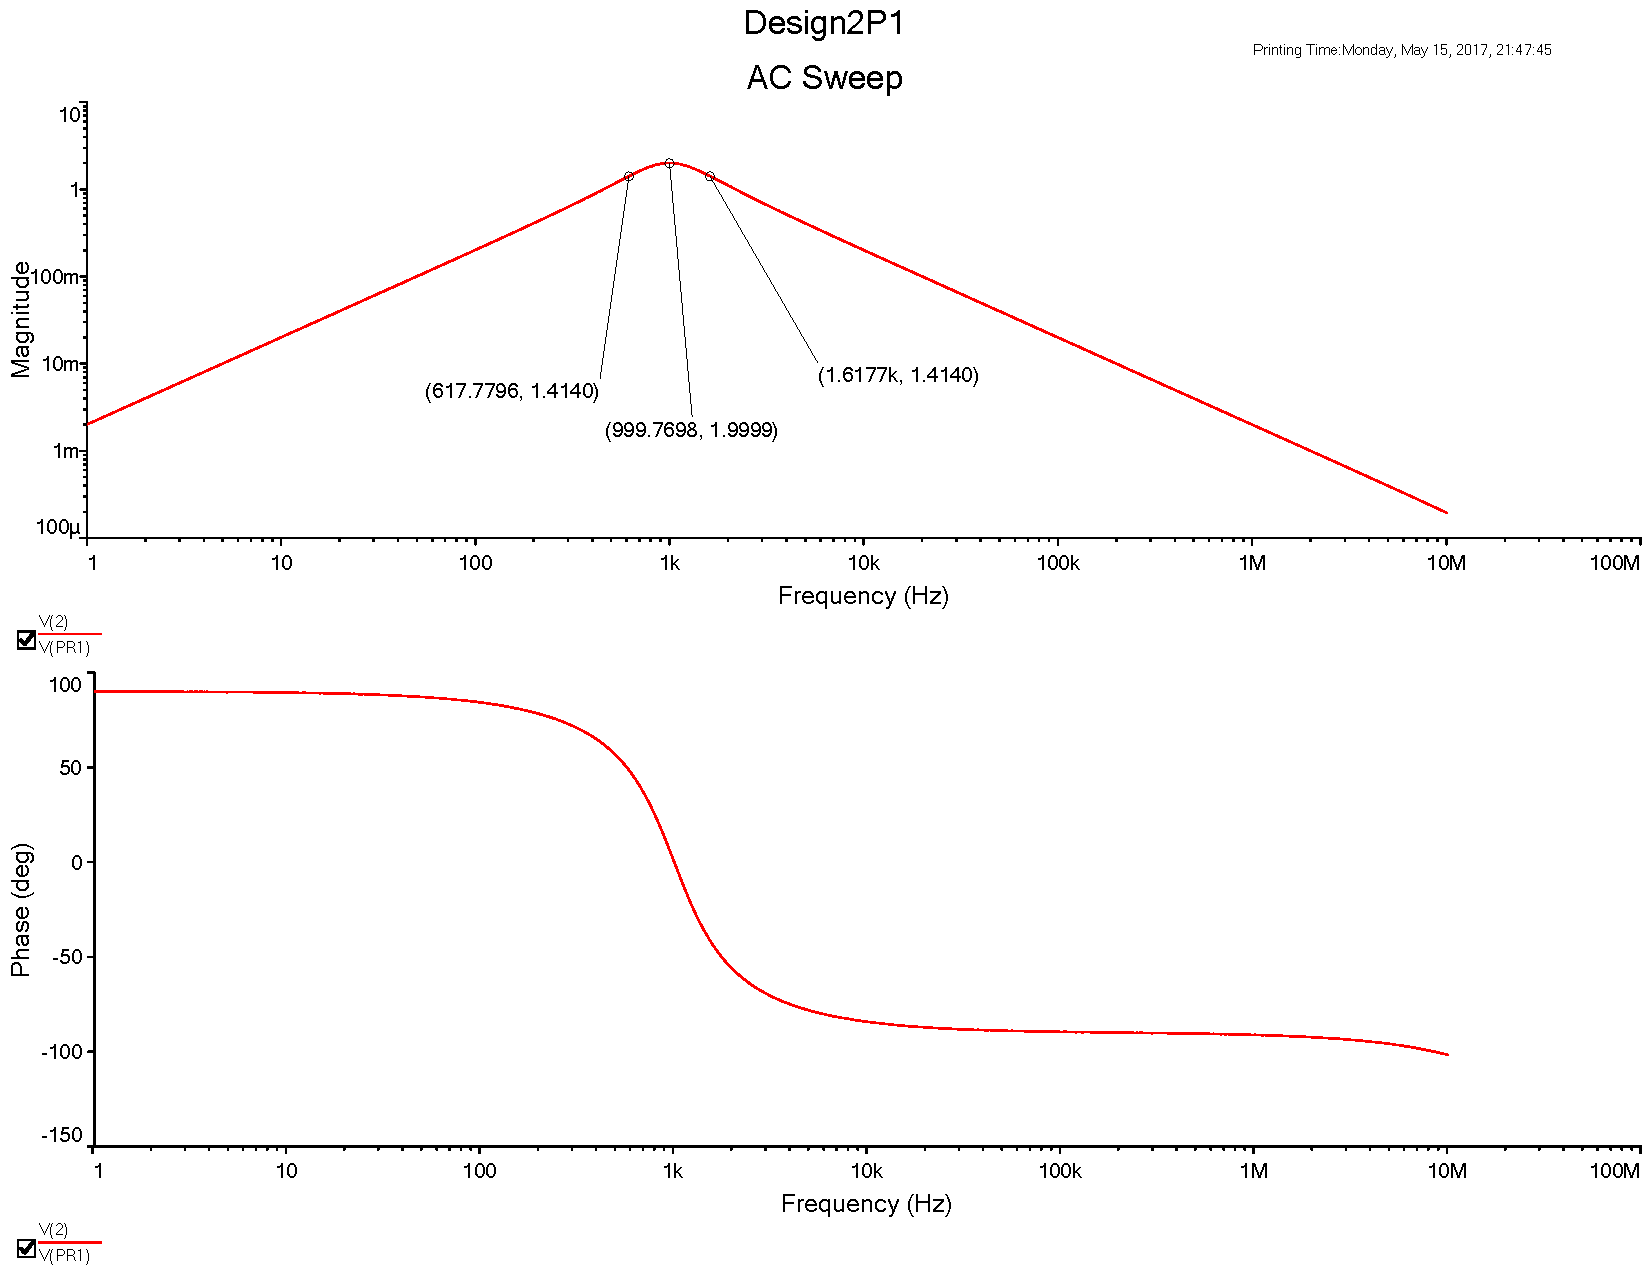
\includegraphics[width=\columnwidth]{2P1.pdf}
\caption{$Q=1$}
\label{LQ1}
\end{figure}
\begin{figure}[H]
\centering
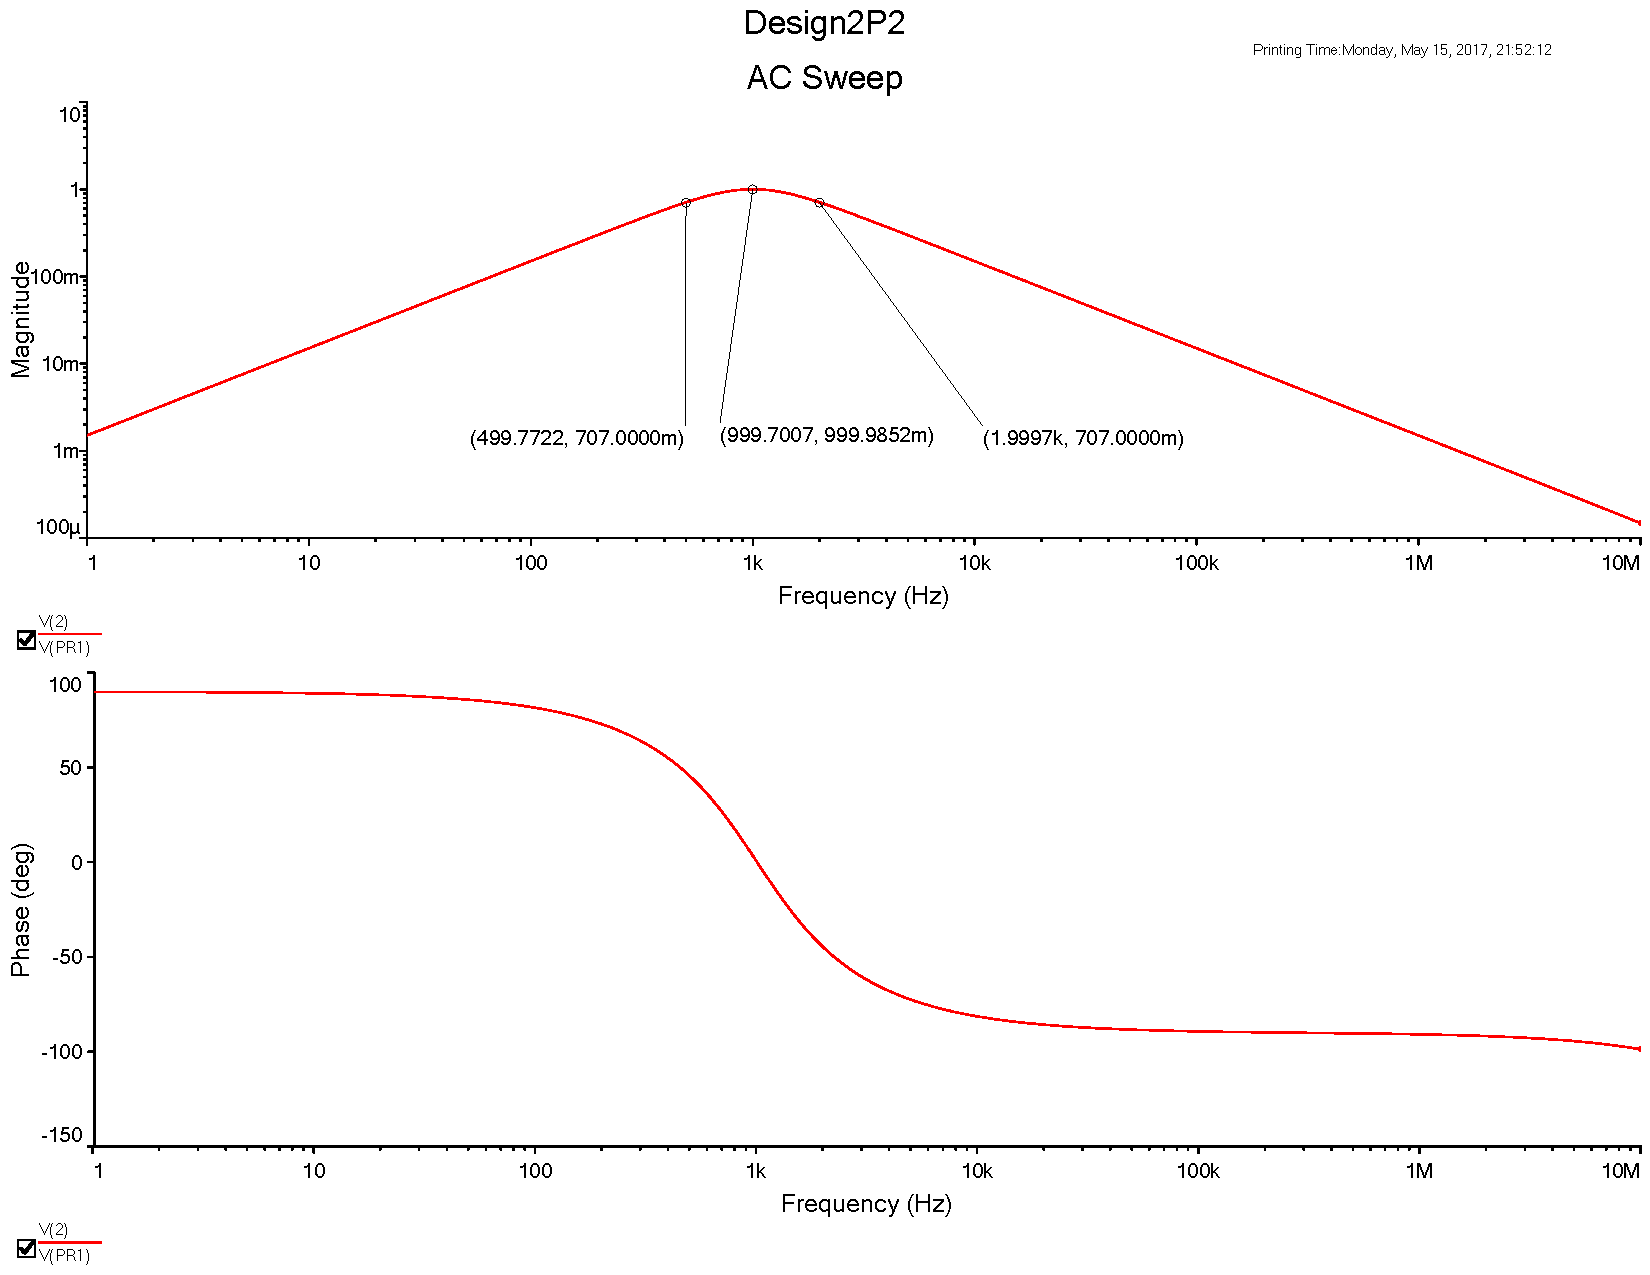
\includegraphics[width=\columnwidth]{2P2_3.pdf}
\caption{$Q=2/3$}
\label{PQ23}
\end{figure}
\begin{figure}[H]
\centering
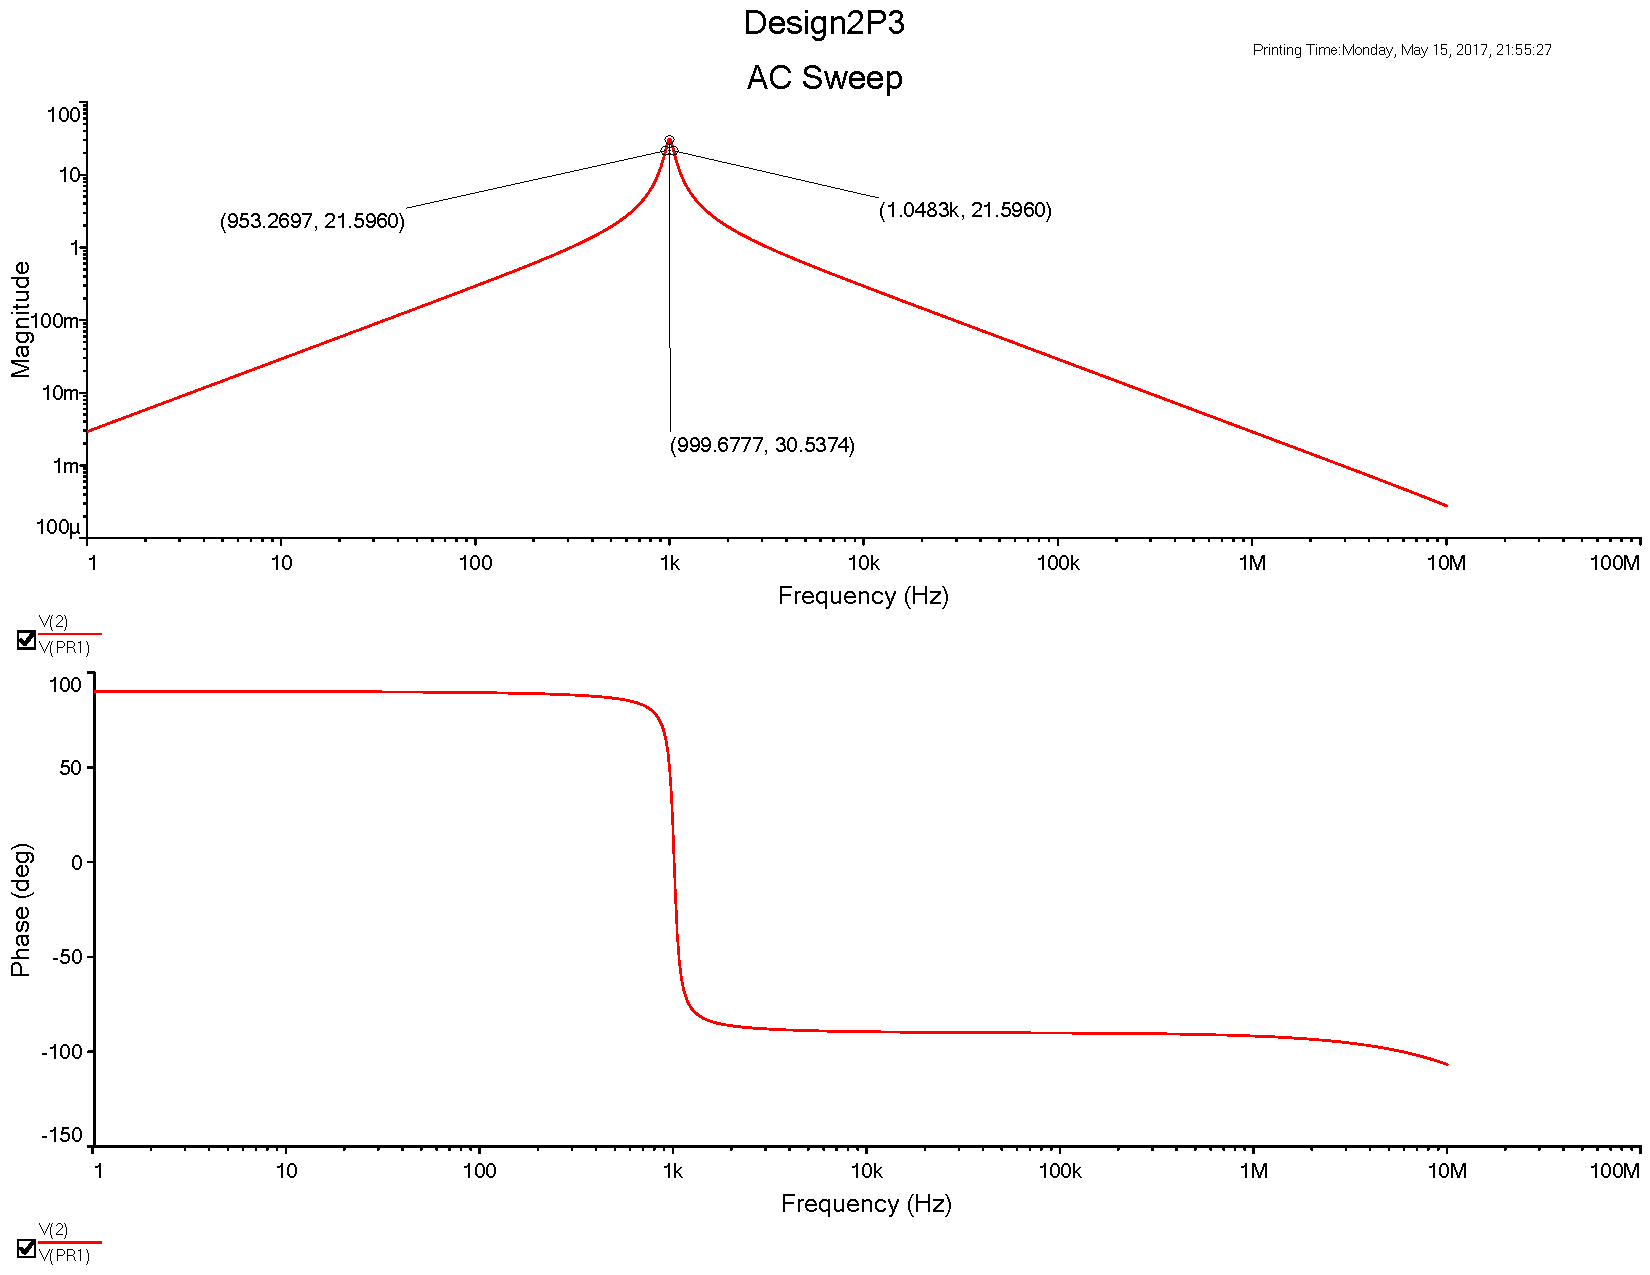
\includegraphics[width=\columnwidth]{2P10_5.pdf}
\caption{$Q=10.5$}
\label{PQ10}
\end{figure}
\begin{figure}[H]
\centering
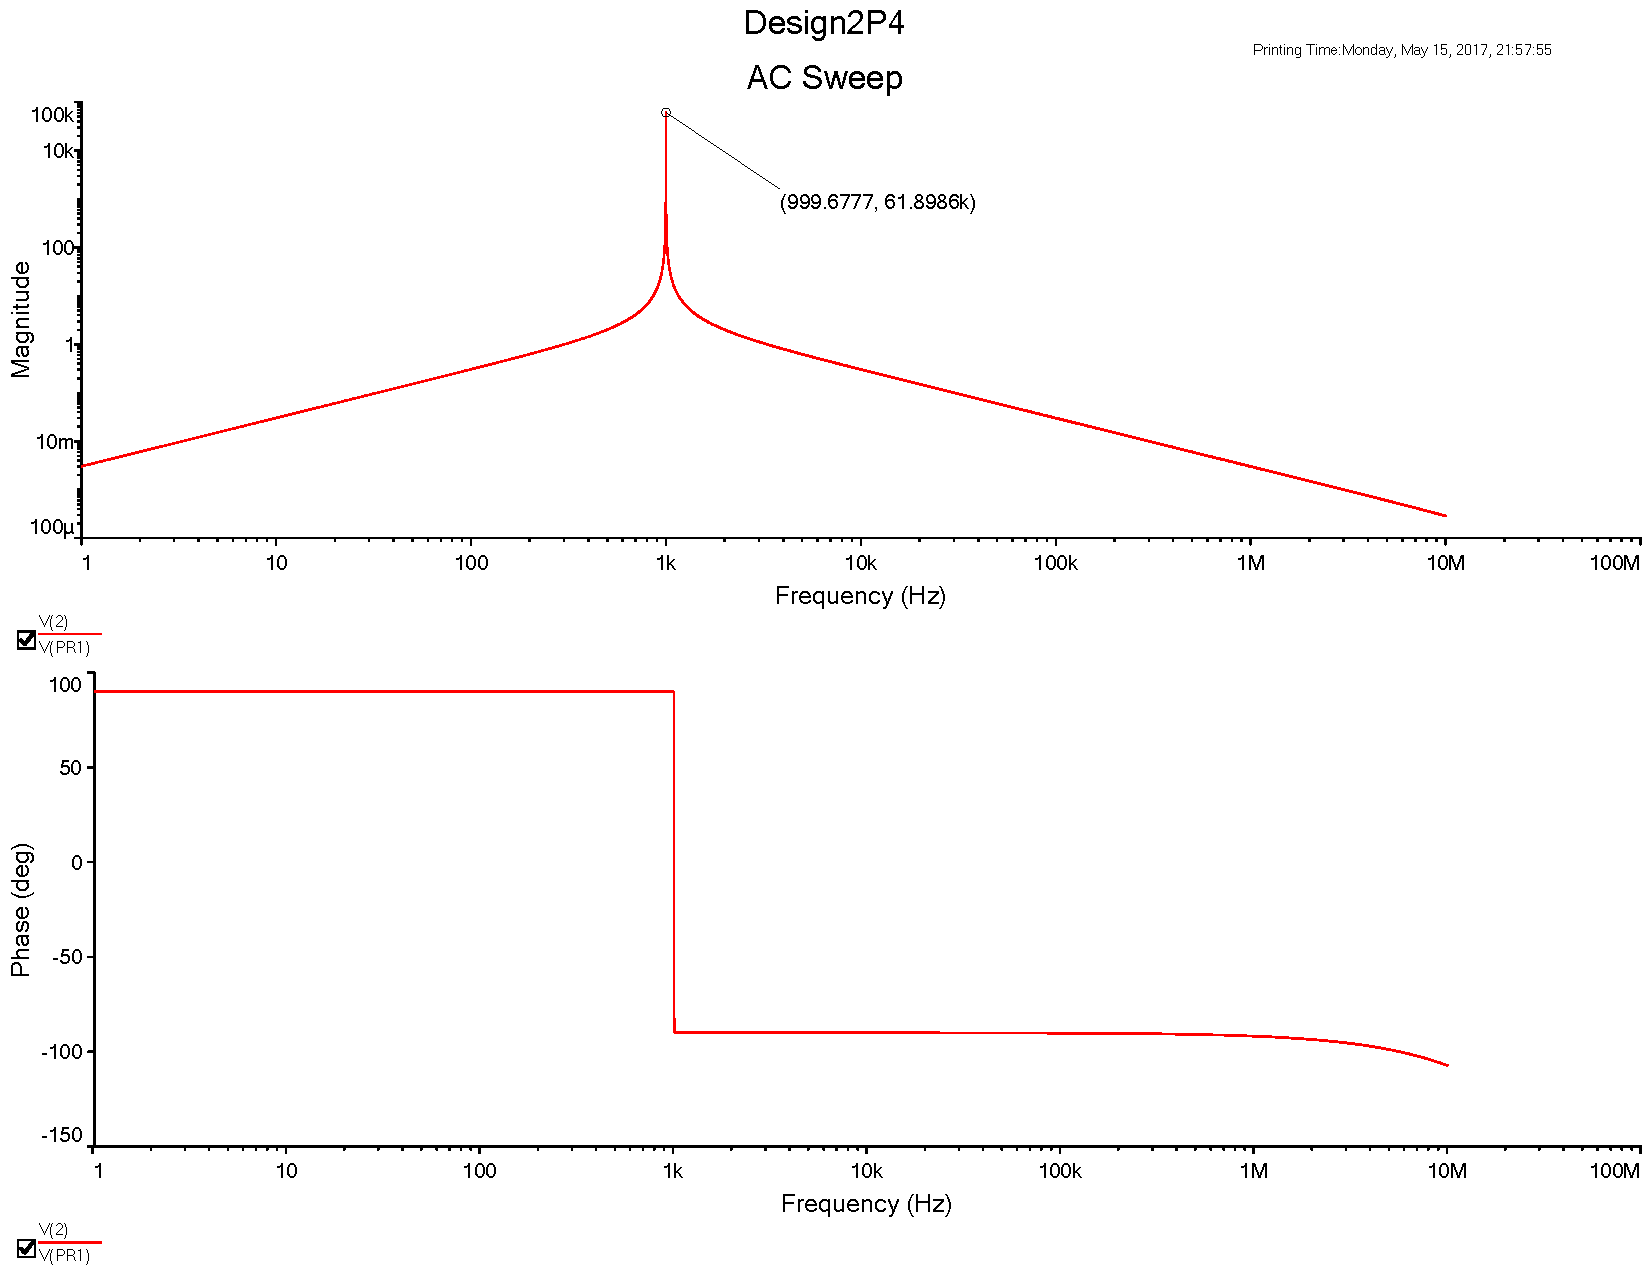
\includegraphics[width=\columnwidth]{2Pinf.pdf}
\caption{$Q=\infty$}
\label{PQinf}
\end{figure}
\begin{figure}[H]
\centering
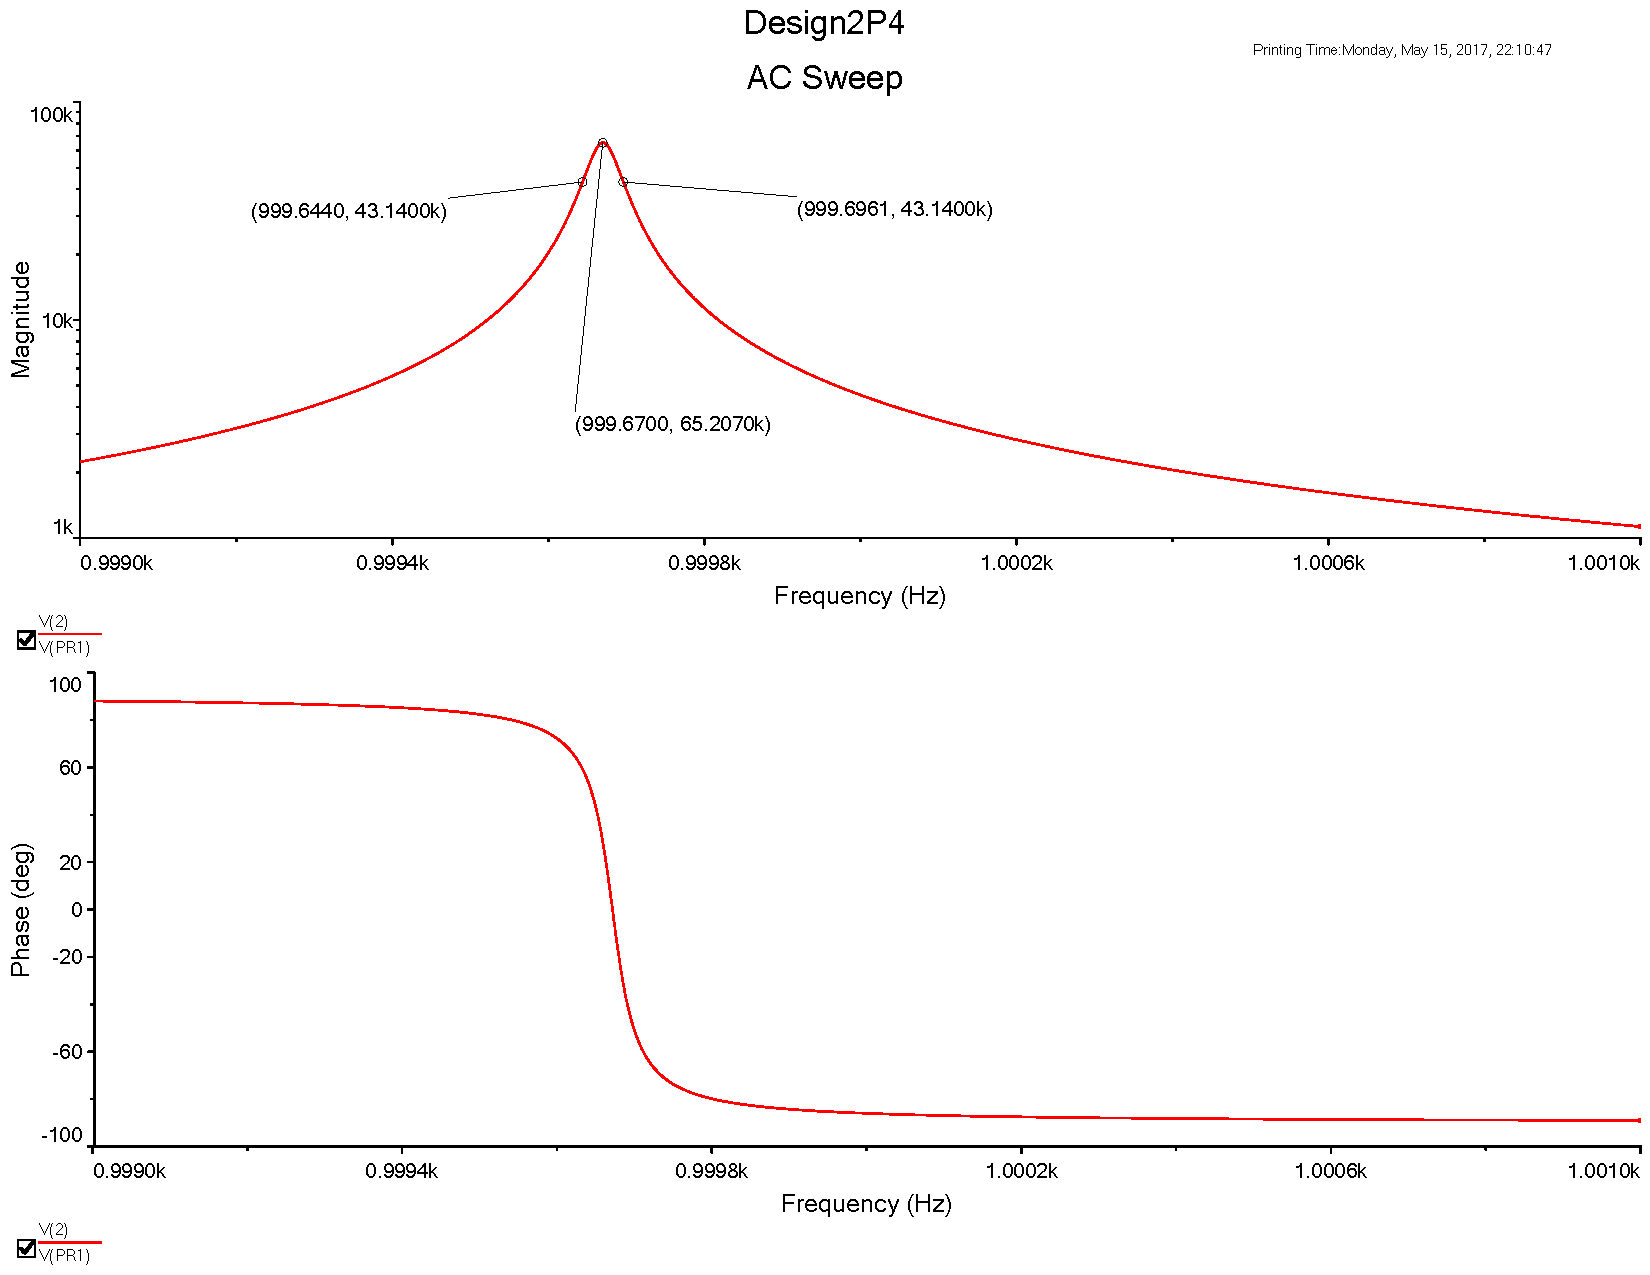
\includegraphics[width=\columnwidth]{2Pinf_1.pdf}
\caption{$Q=\infty$细节特性}
\label{PQinf1}
\end{figure}
\begin{table}[H]
\centering
\label{table1}
\caption{带宽和$Q$值的变化关系}
\begin{tabular}{ll}
\hline
$Q$&$f_w/\mathrm{Hz}$\\
\hline
$\frac{2}{3}$&1500\\
1&1000\\
10.5&95.03\\
$\infty$&0.05\\
\hline
\end{tabular}
\end{table}
\end{multicols}
可以看到,带通滤波器的相频曲线从180逐渐变为-180,随着Q值的增大,相变的位置逐渐收敛到特征频率$f_0$的位置,使得相频特性更加趋近于一个阶跃函数的形式。

同时,也可以看到,随着$Q$值的增大,电路的选频特性不断增加,但频带宽度逐渐减小,我们可以总结为表\ref{table1},可以验证基本满足$f_w=\frac{f_0}{Q}$的理论结果,说明电路 是合理的。

\subsubsection{倒T型网络带阻滤波器搭建和测试}
采用经典设计了倒T型网络VCVS带阻滤波器,设计得到特征频率为1kHz,其bode图如下图所示,其中设定了$Q=\infty$方便分析,可以猜想频率响应随Q的变化和前几个基本相同。

相频上电路从0到0变化,在特征频率上出现了明显的同相-反相翻转。
\begin{figure}[h]
\centering
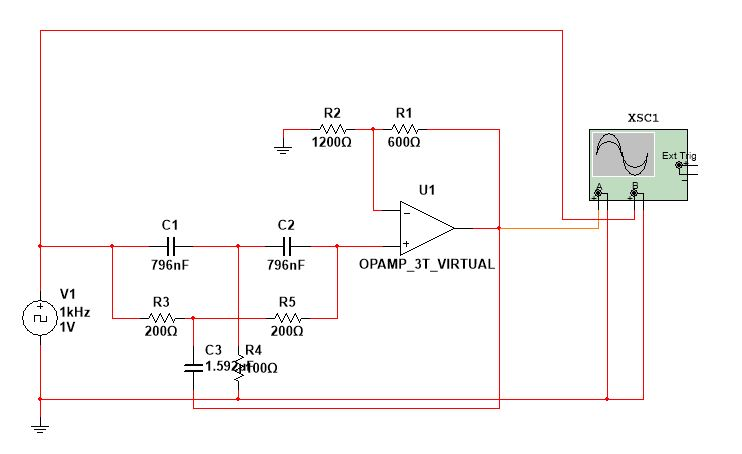
\includegraphics[width=\columnwidth]{S.jpg}
\caption{倒T型网络带阻滤波电路}
\label{P}
\end{figure}
\begin{multicols}{2}
\begin{figure}[H]
\centering
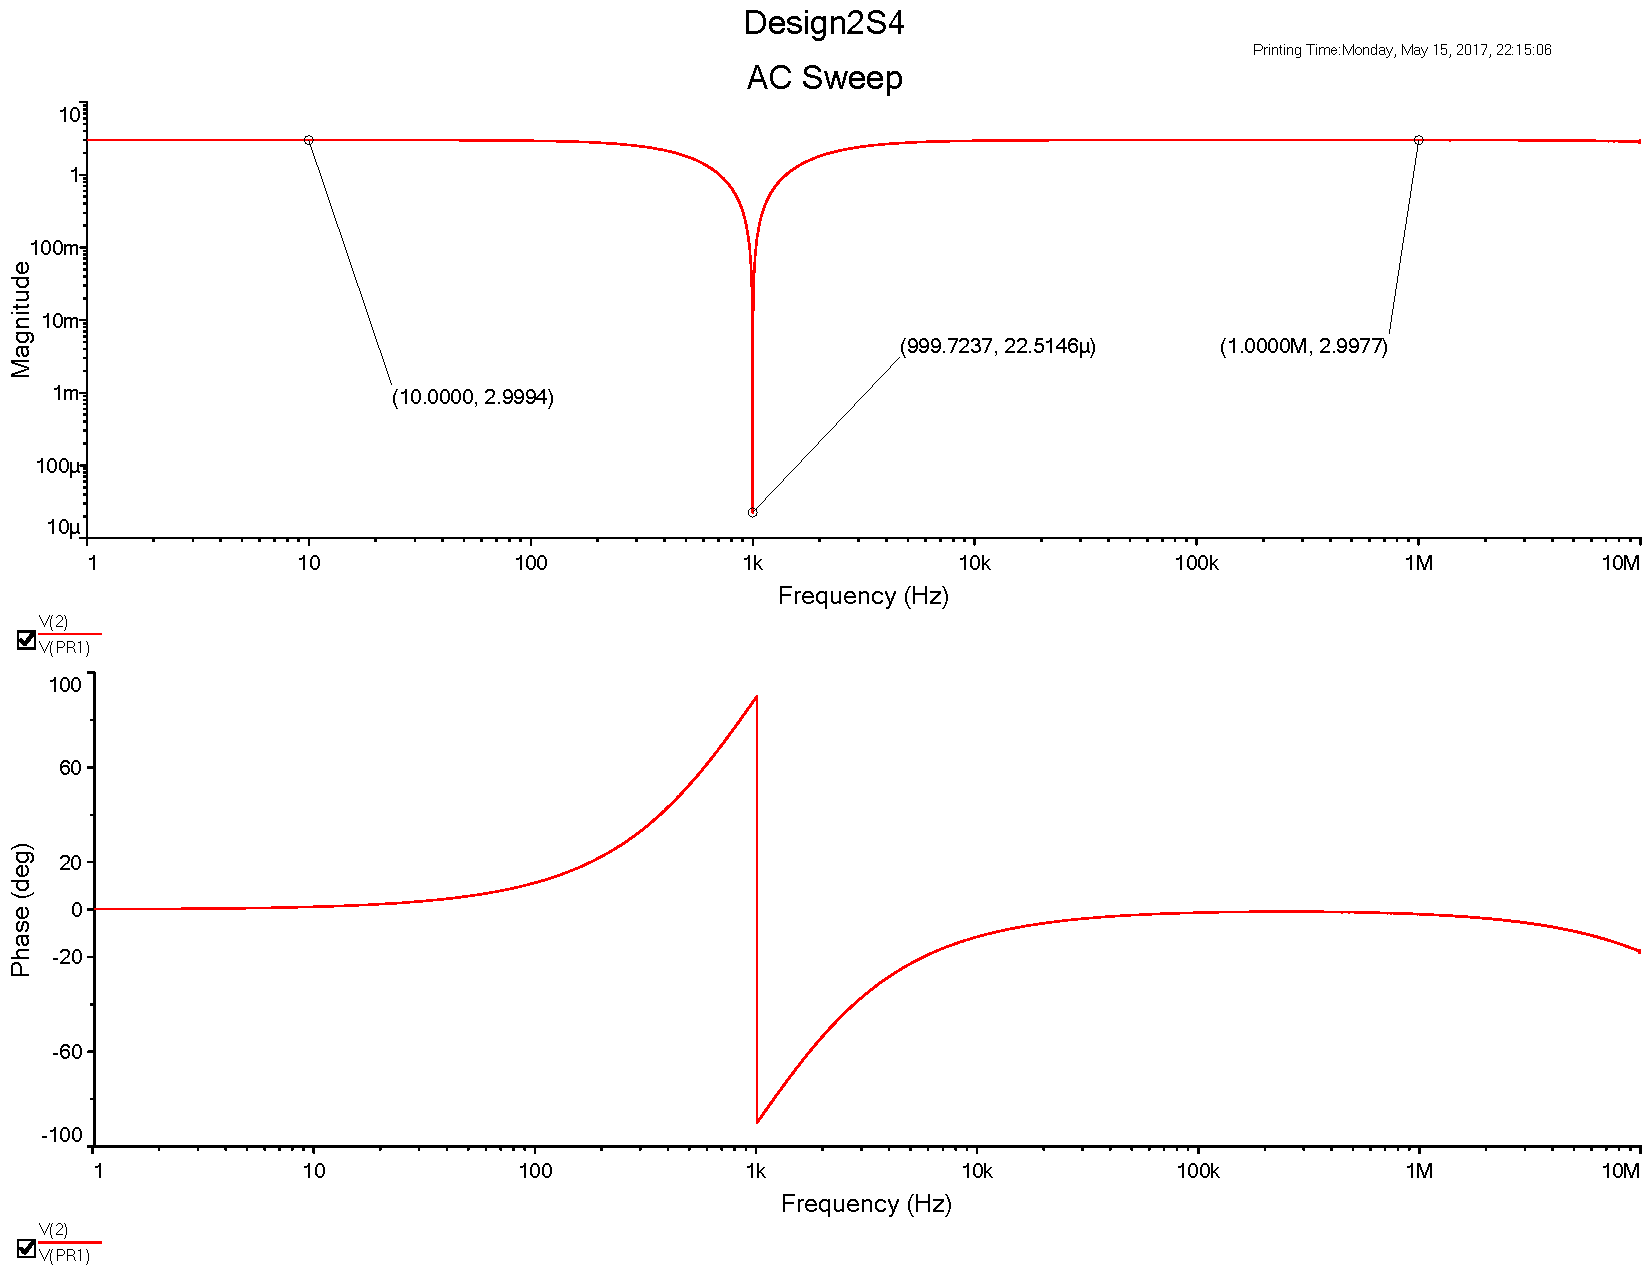
\includegraphics[width=\columnwidth]{2Sinf.pdf}
\caption{倒T型网络带阻滤波频率特性}
\label{SQ}
\end{figure}
\begin{figure}[H]
\centering
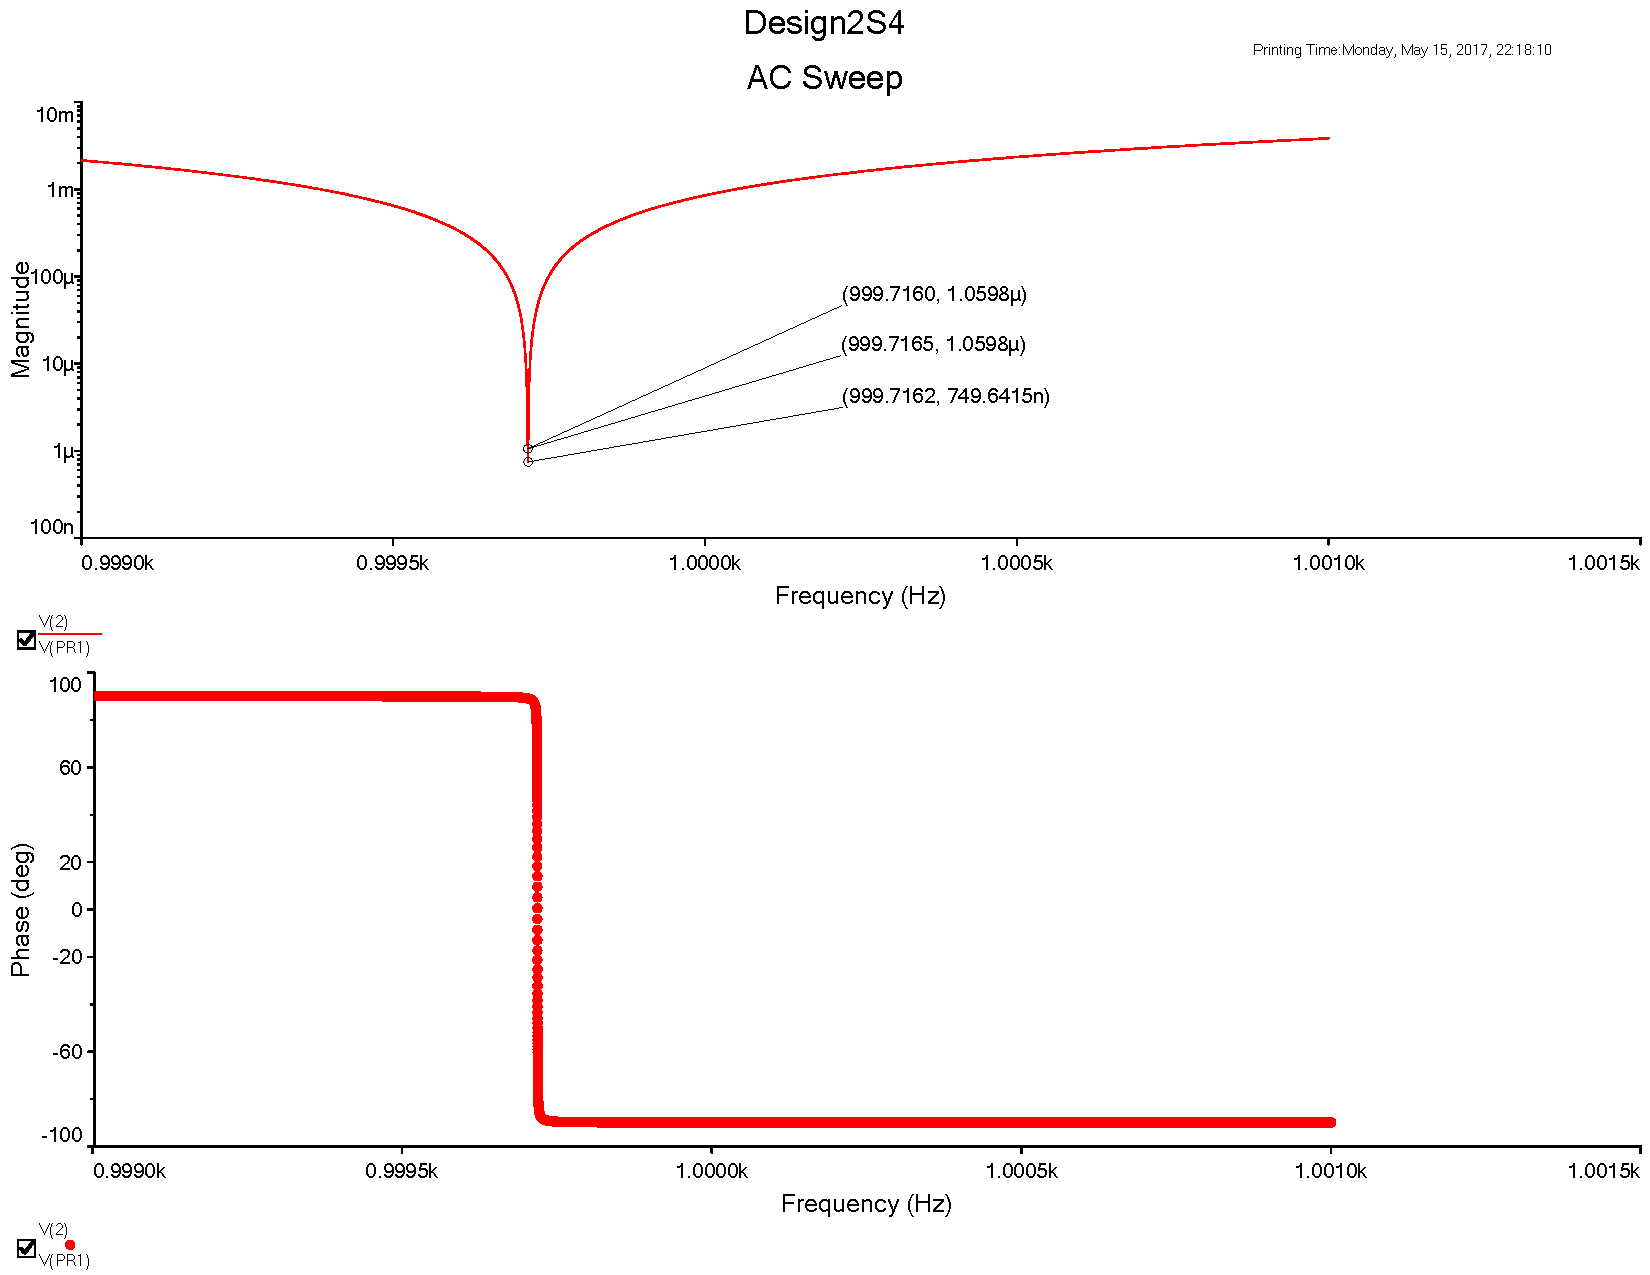
\includegraphics[width=\columnwidth]{2Sinf_1.pdf}
\caption{倒T型网络带阻滤波器频率特性细节}
\label{SQ1}
\end{figure}
\end{multicols}
\begin{multicols}{2}
\subsection{输出波形的研究}
通过输入方波来研究四个网络的频率特性,从理论上我们可以看出,直流分量是低频成分的代表而边沿陡峭的波形是高频成分的代表。从波形的这两个特性上我们就可以对滤波器的频率特性有一定的了解。
\subsubsection{低通滤波器波形研究}
如图\ref{BIL}所示,我们可以看到波形存在明显的直流分量并且波形平滑,可以推出滤波器是低通滤波器,和现实情况相符。
\begin{figure}[H]
\centering
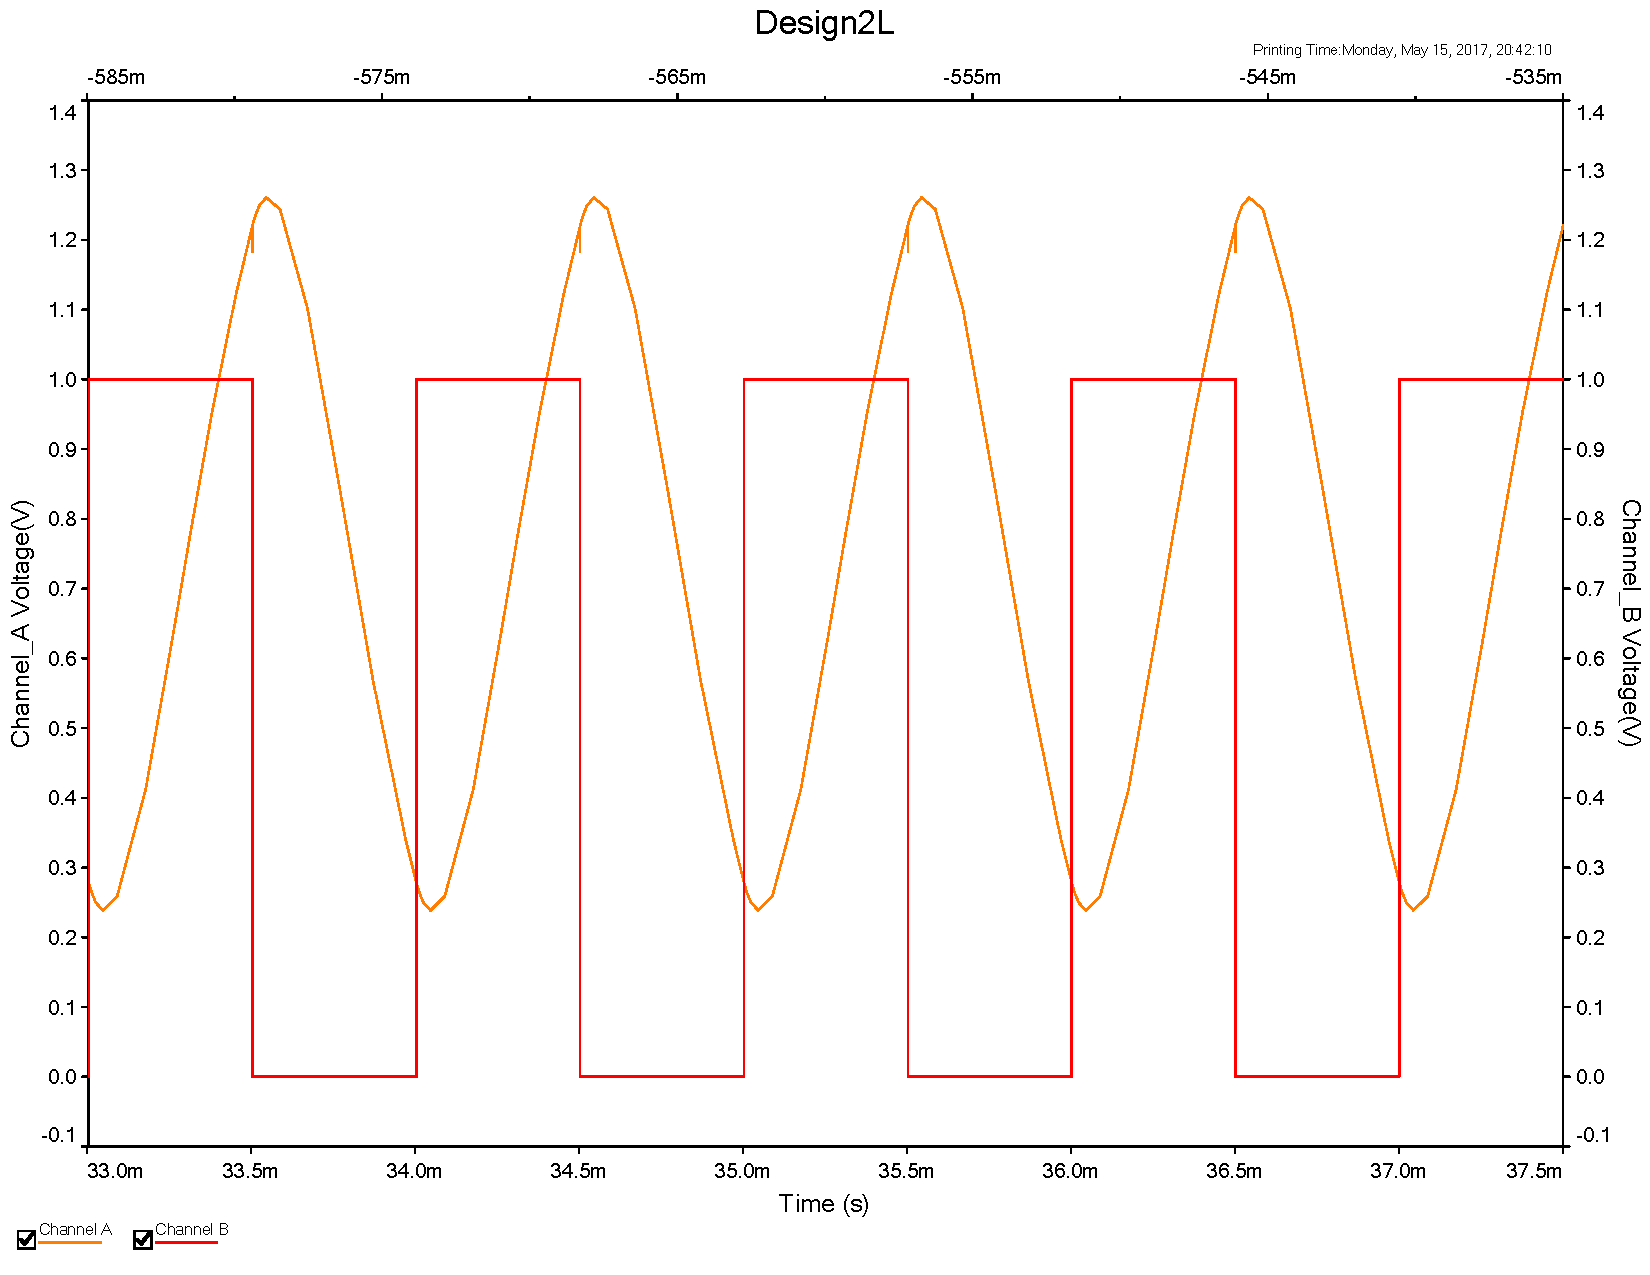
\includegraphics[width=\columnwidth]{2L.pdf}
\caption{方波通过低通滤波器的波形}
\label{BIL}
\end{figure}
\subsubsection{高通滤波器波形研究}
如图\ref{BIH}所示,我们可以看到波形不存在明显的直流分量并且波形陡峭尖峰明显,可以推出滤波器是高通滤波器,和现实情况相符。
\begin{figure}[H]
\centering
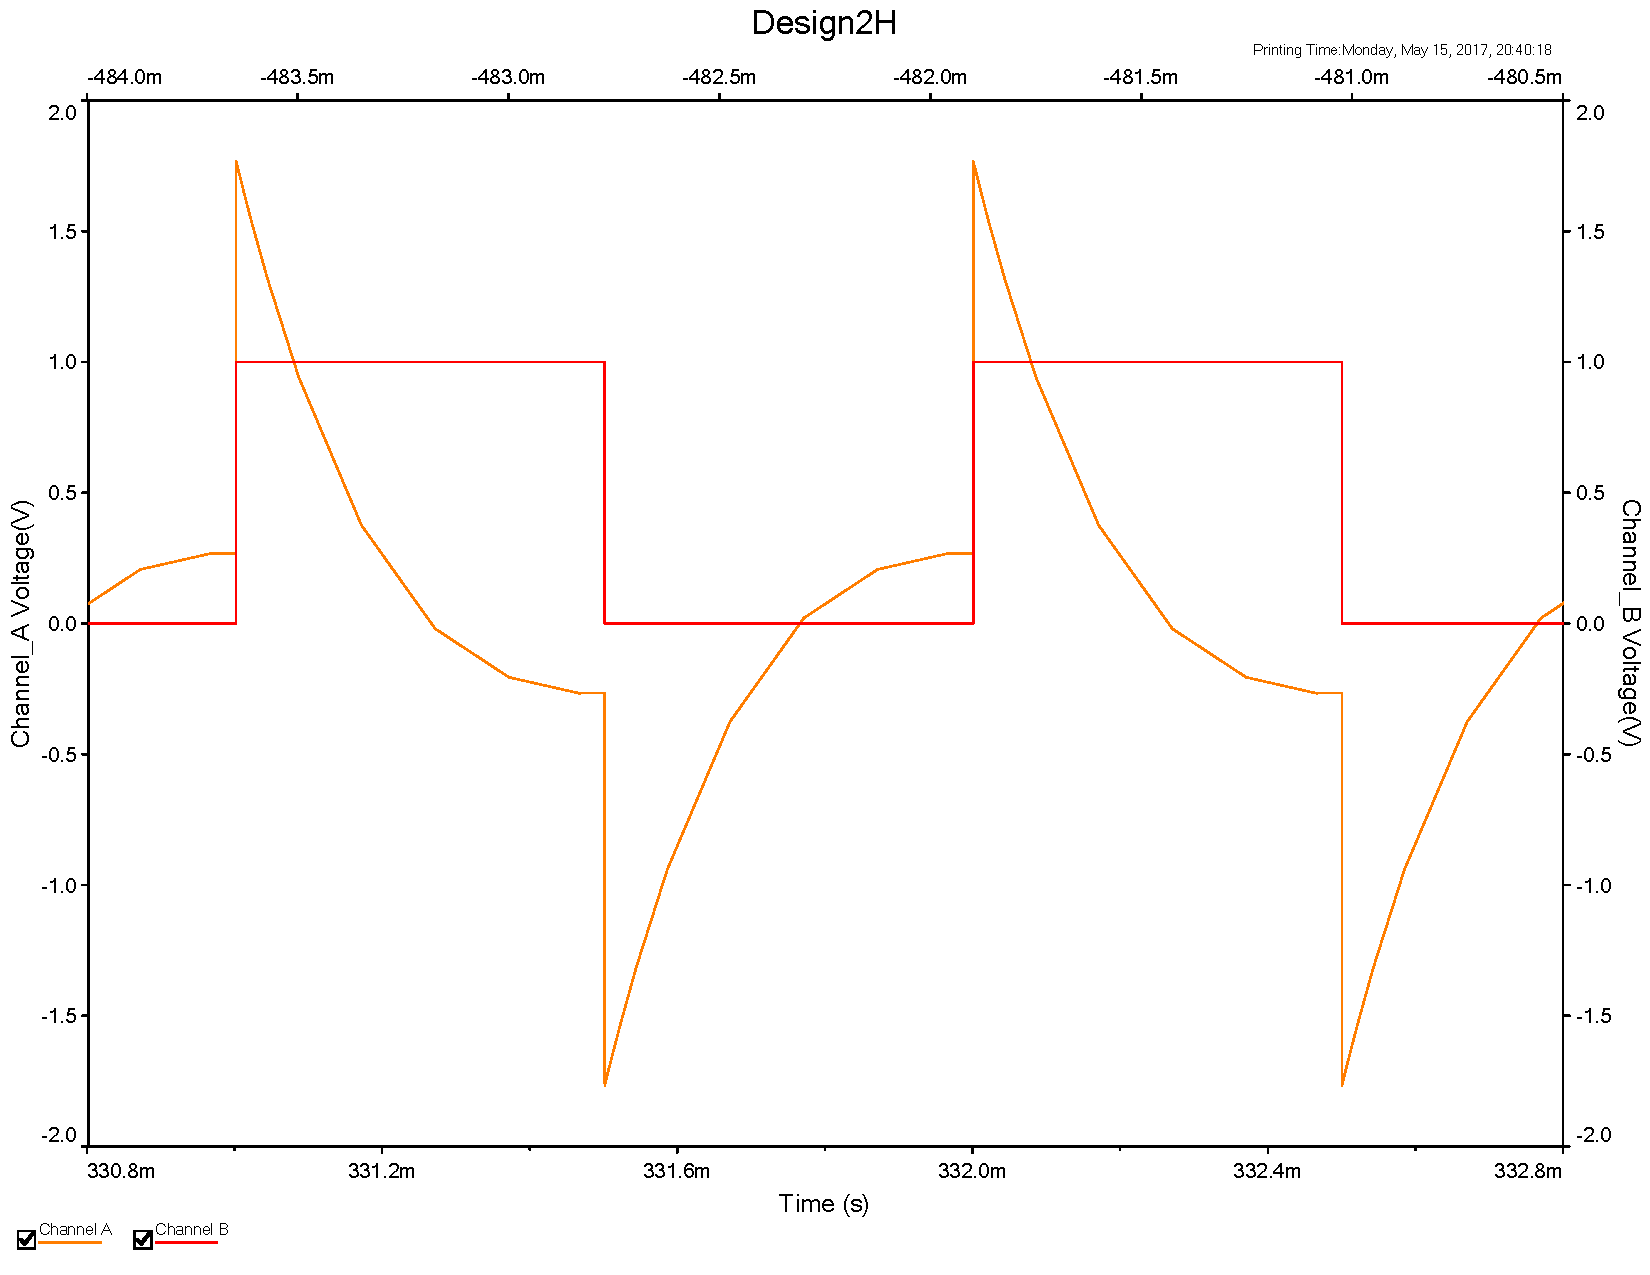
\includegraphics[width=\columnwidth]{2H.pdf}
\caption{方波通过高通滤波器的波形}
\label{BIH}
\end{figure}
\subsubsection{带通滤波器波形研究}
如图\ref{BIP}所示,我们可以看到波形不存在明显的直流分量并且波形平滑,可以推出滤波器是带通滤波器,和现实情况相符。
\begin{figure}[H]
\centering
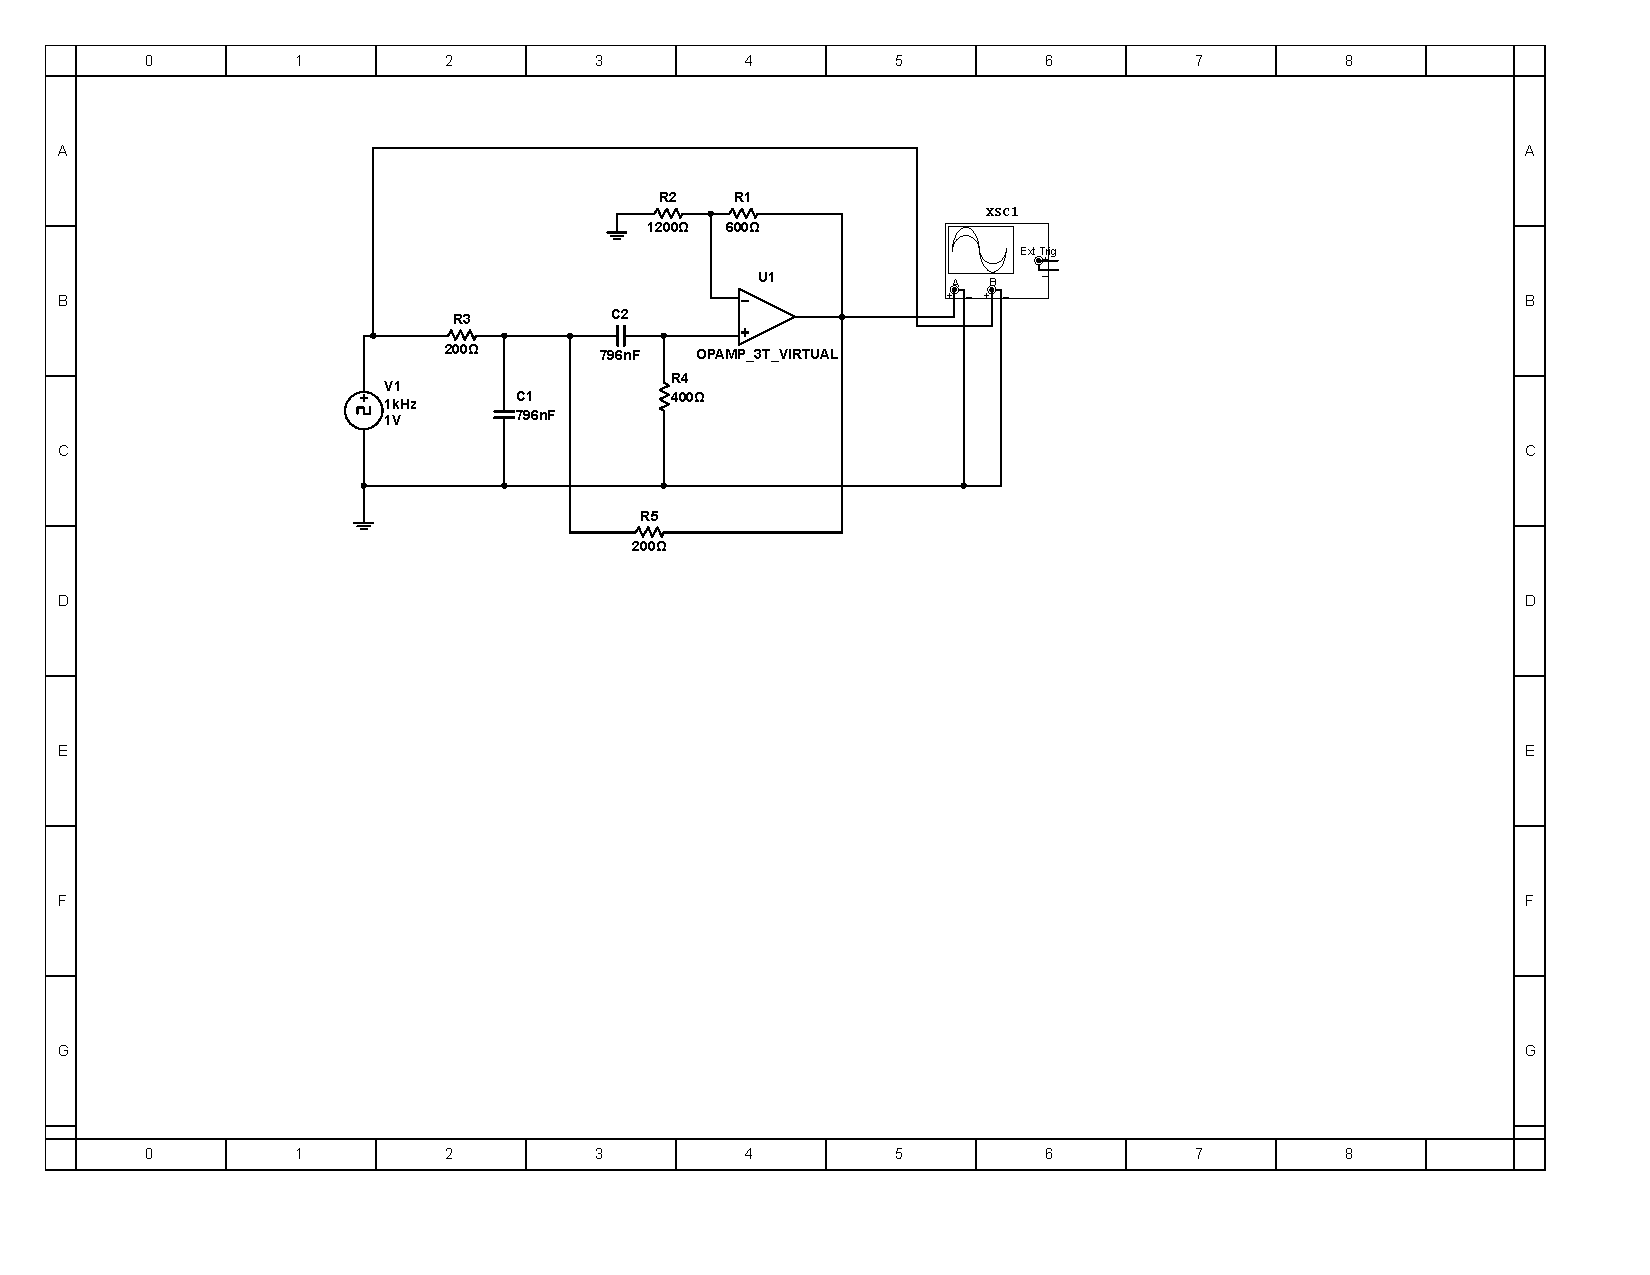
\includegraphics[width=\columnwidth]{2P.pdf}
\caption{方波通过带通滤波器的波形}
\label{BIP}
\end{figure}
\subsubsection{带阻滤波器波形研究}
如图\ref{BIS}所示,我们可以看到波形存在明显的直流分量并且波形波形陡峭尖峰明显,可以推出滤波器是带阻滤波器,和现实情况相符。
\begin{figure}[H]
\centering
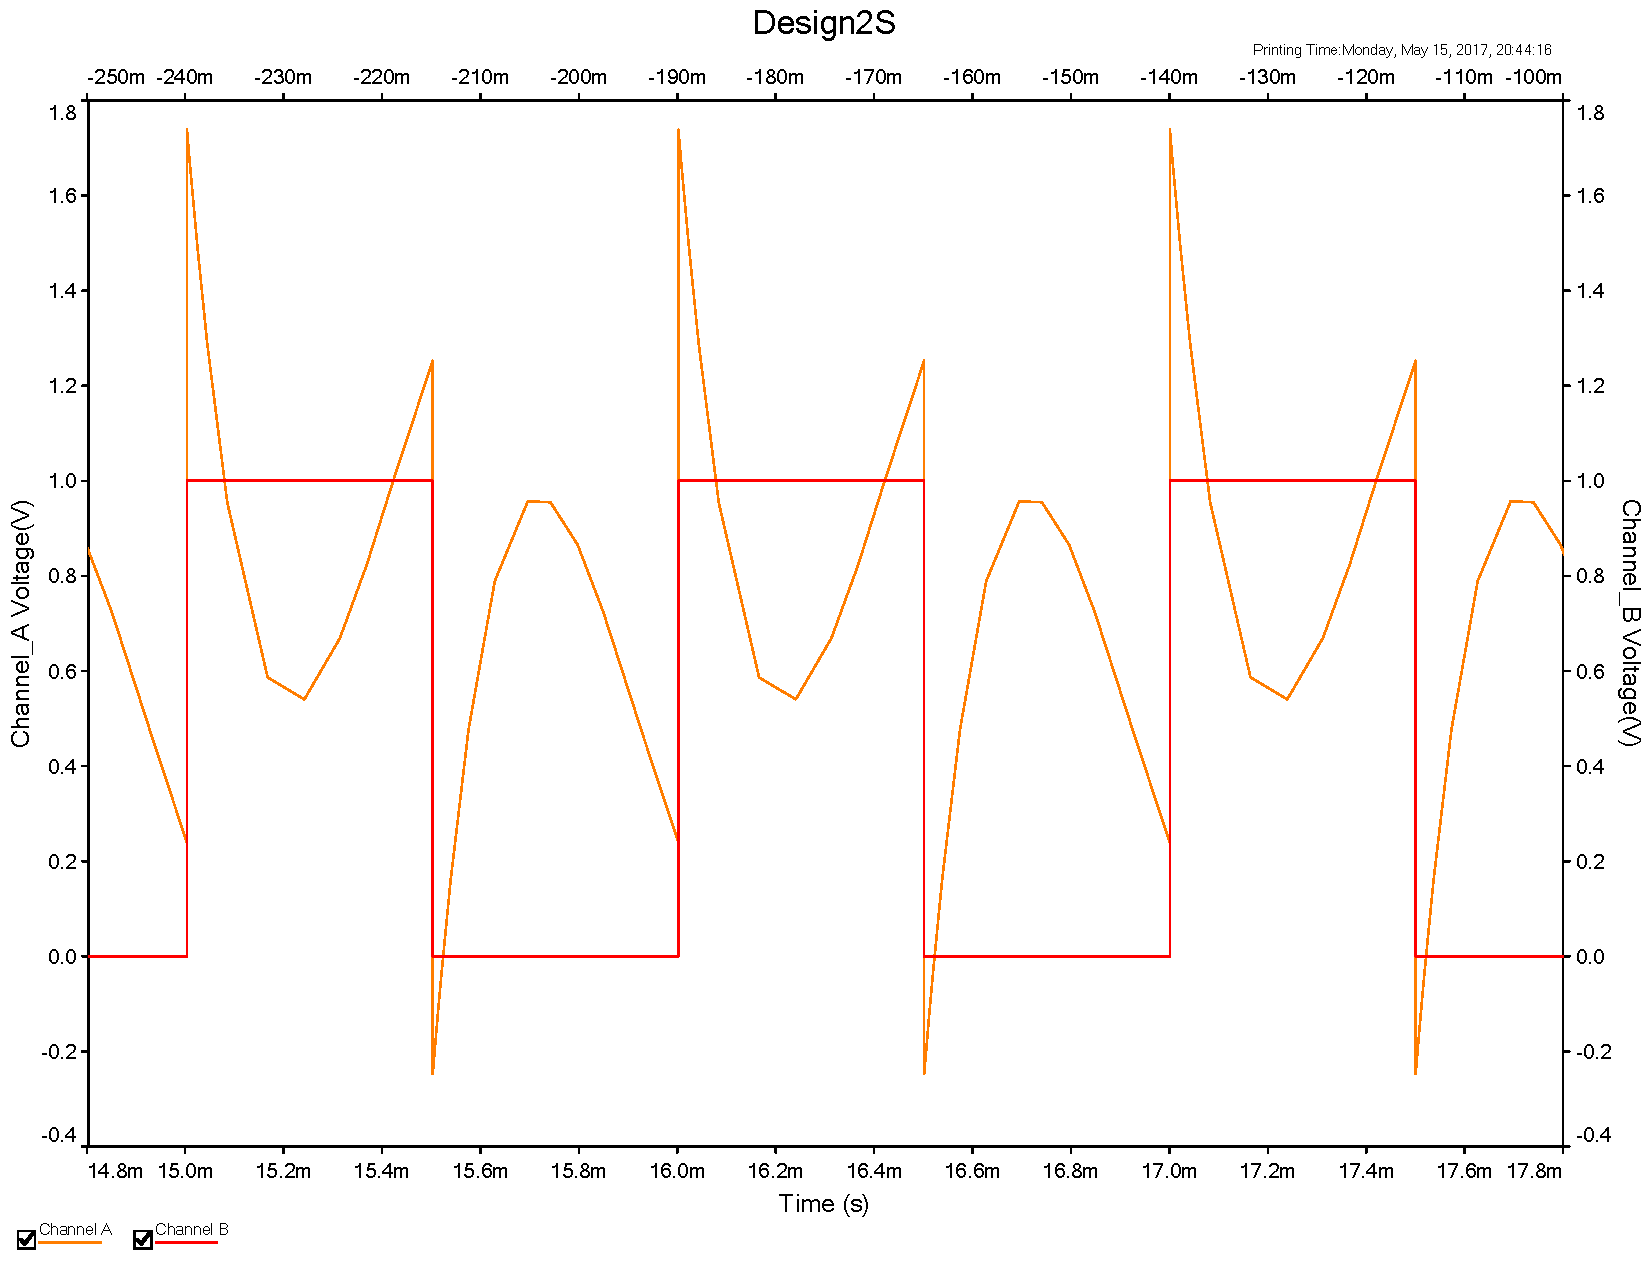
\includegraphics[width=\columnwidth]{2S.pdf}
\caption{方波通过带阻滤波器的波形}
\label{BIS}
\end{figure}
\subsection{不稳定滤波器的波形}
对于$Q>3$的滤波器,我们可以看到他是不稳定的,因此在信号激励下会迅速到达运放摆幅进行震荡,而如图\ref{BILF},\ref{BIHF},\ref{BIPF},\ref{BISF}所示,对四个滤波器来说是相同的效果。
\begin{figure}[H]
\centering
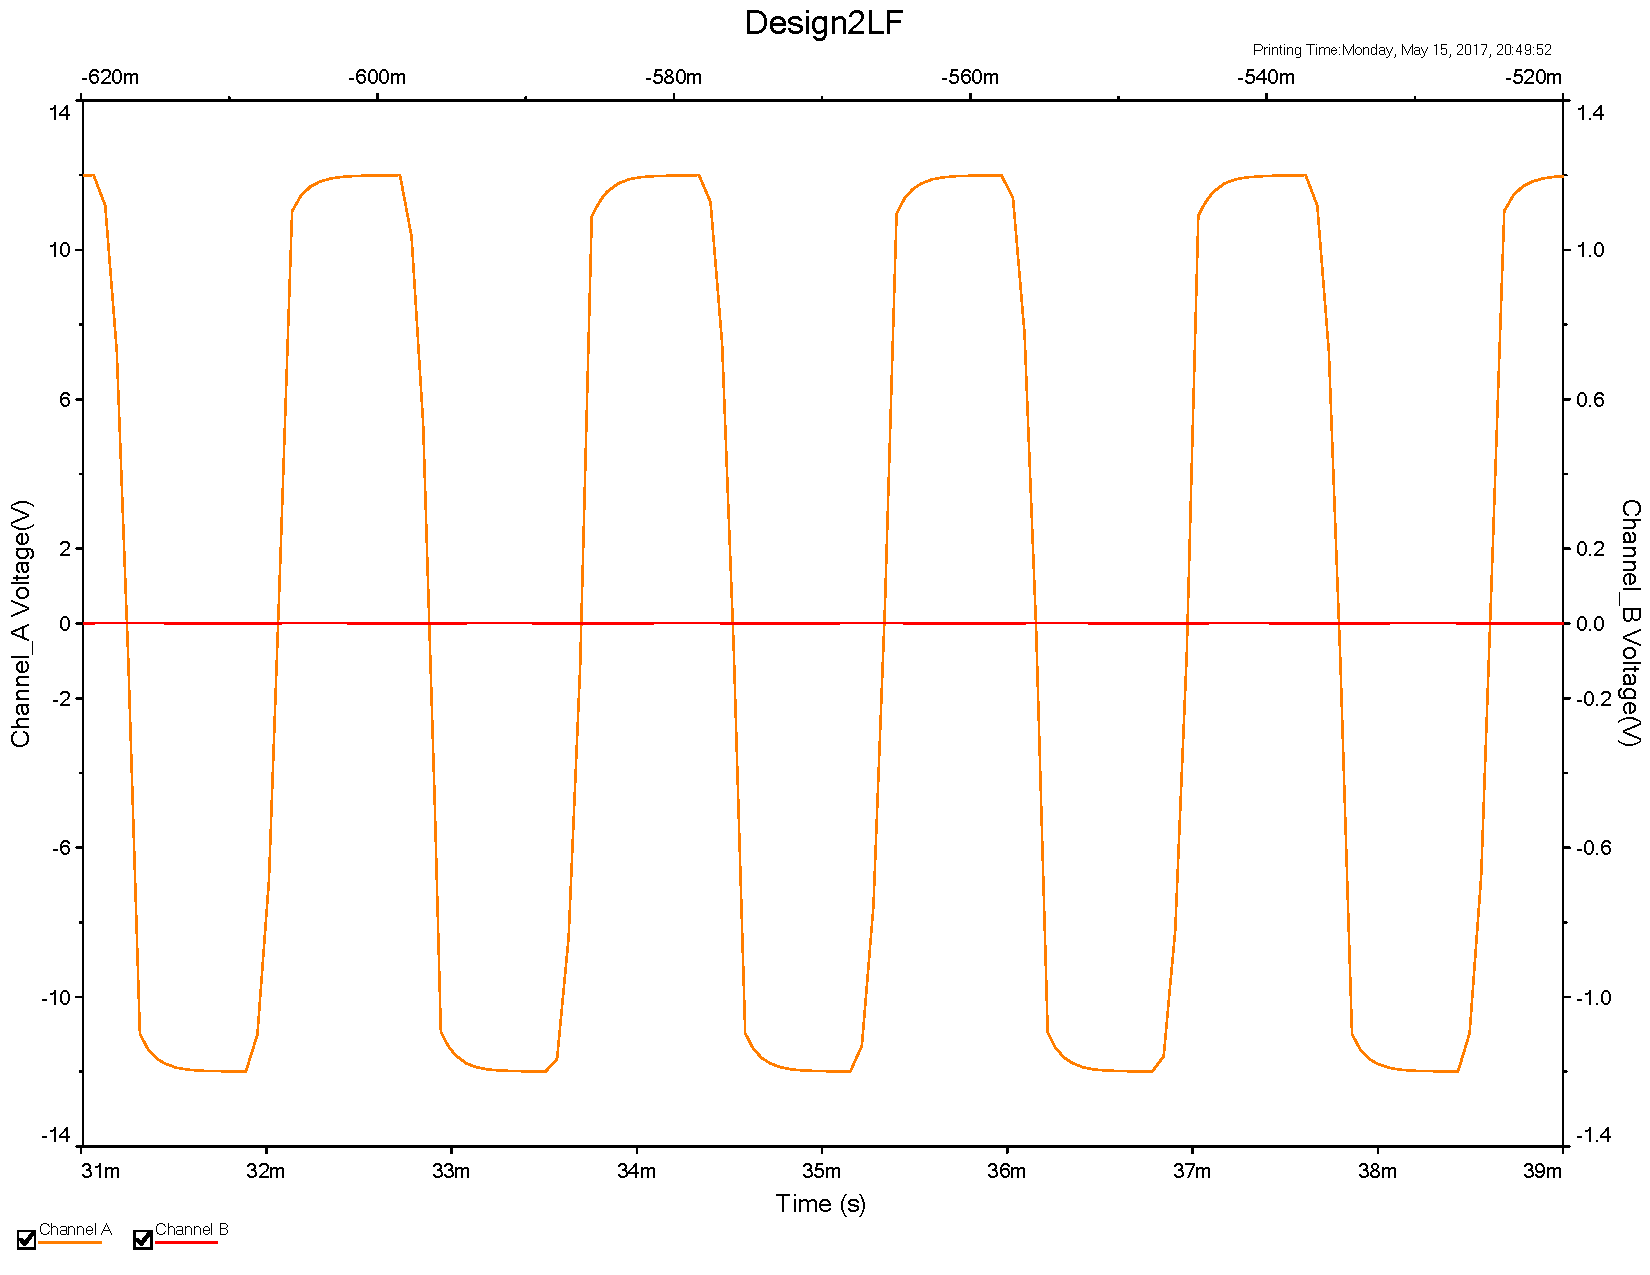
\includegraphics[width=\columnwidth]{2LF.pdf}
\caption{低通滤波器不稳定波形}
\label{BILF}
\end{figure}
\begin{figure}[H]
\centering
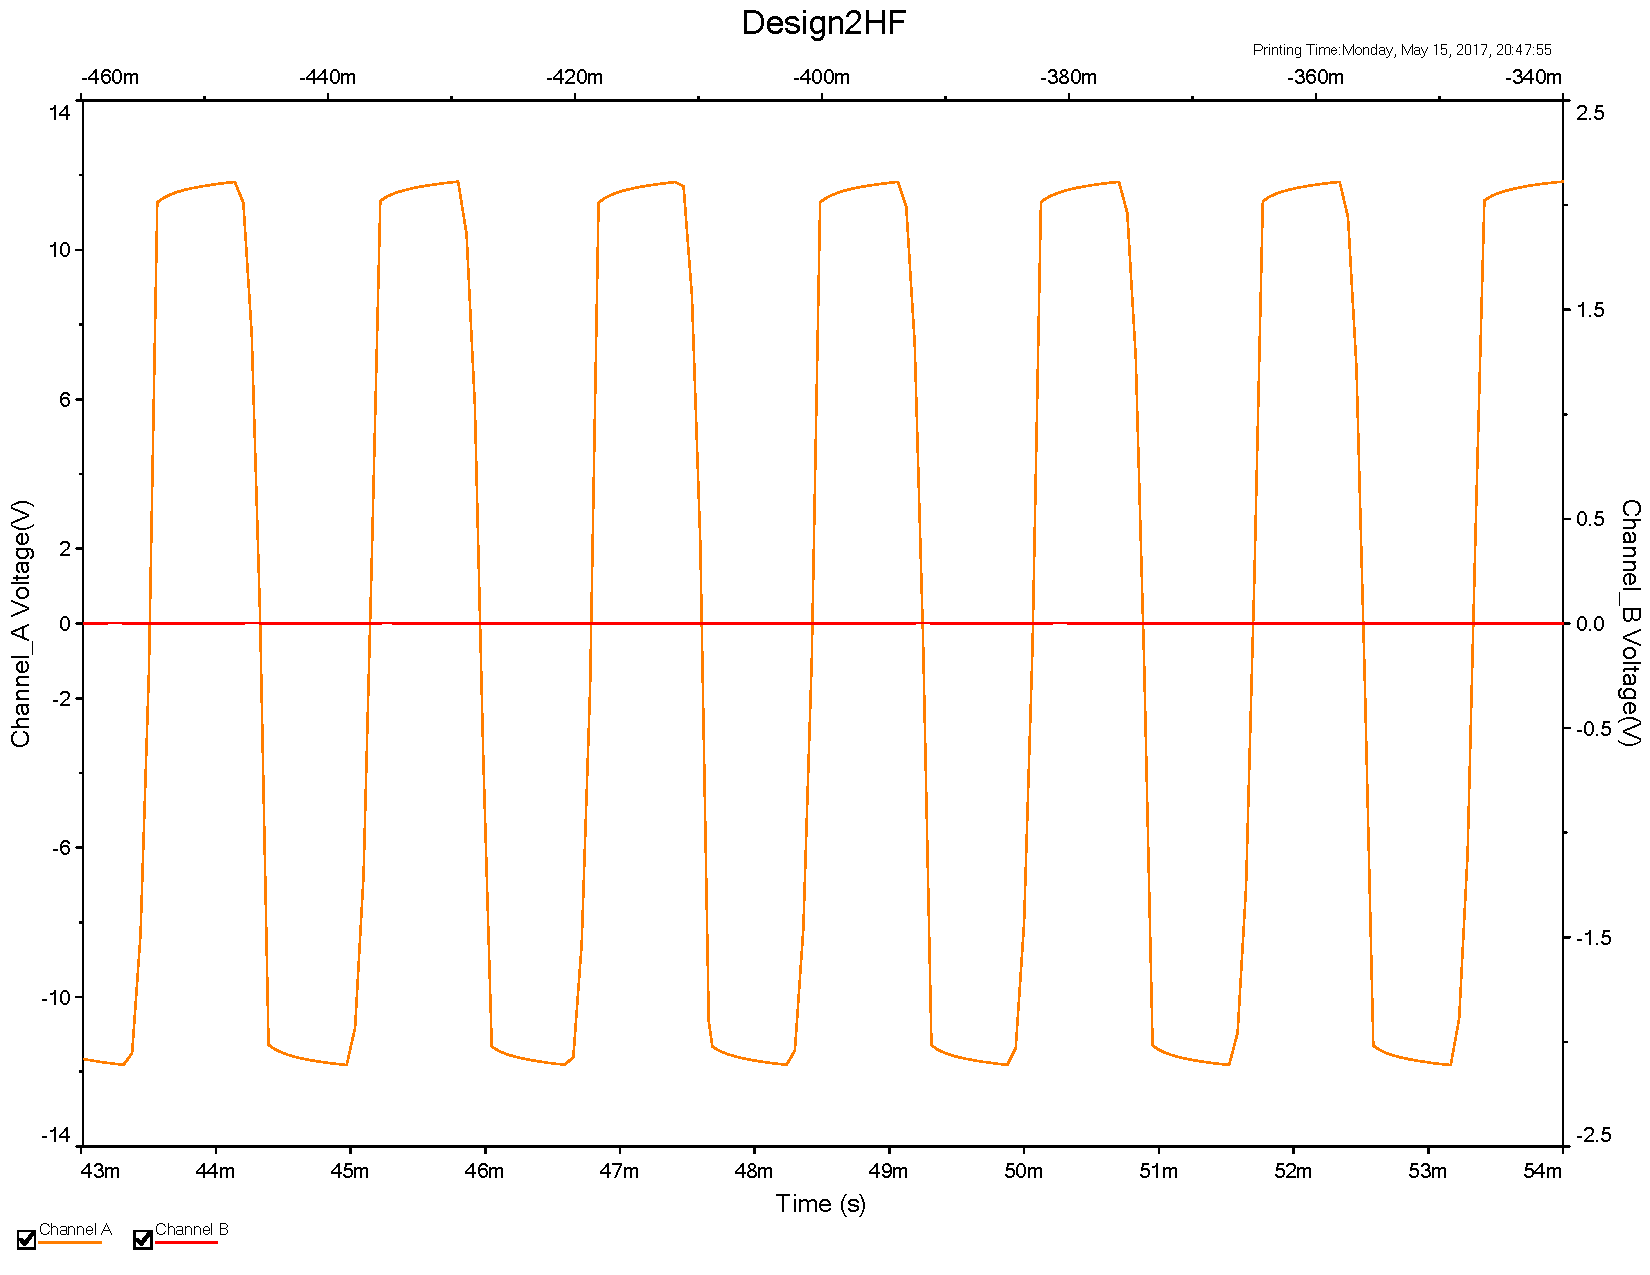
\includegraphics[width=\columnwidth]{2HF.pdf}
\caption{高通滤波器不稳定波形}
\label{BIHF}
\end{figure}
\begin{figure}[H]
\centering
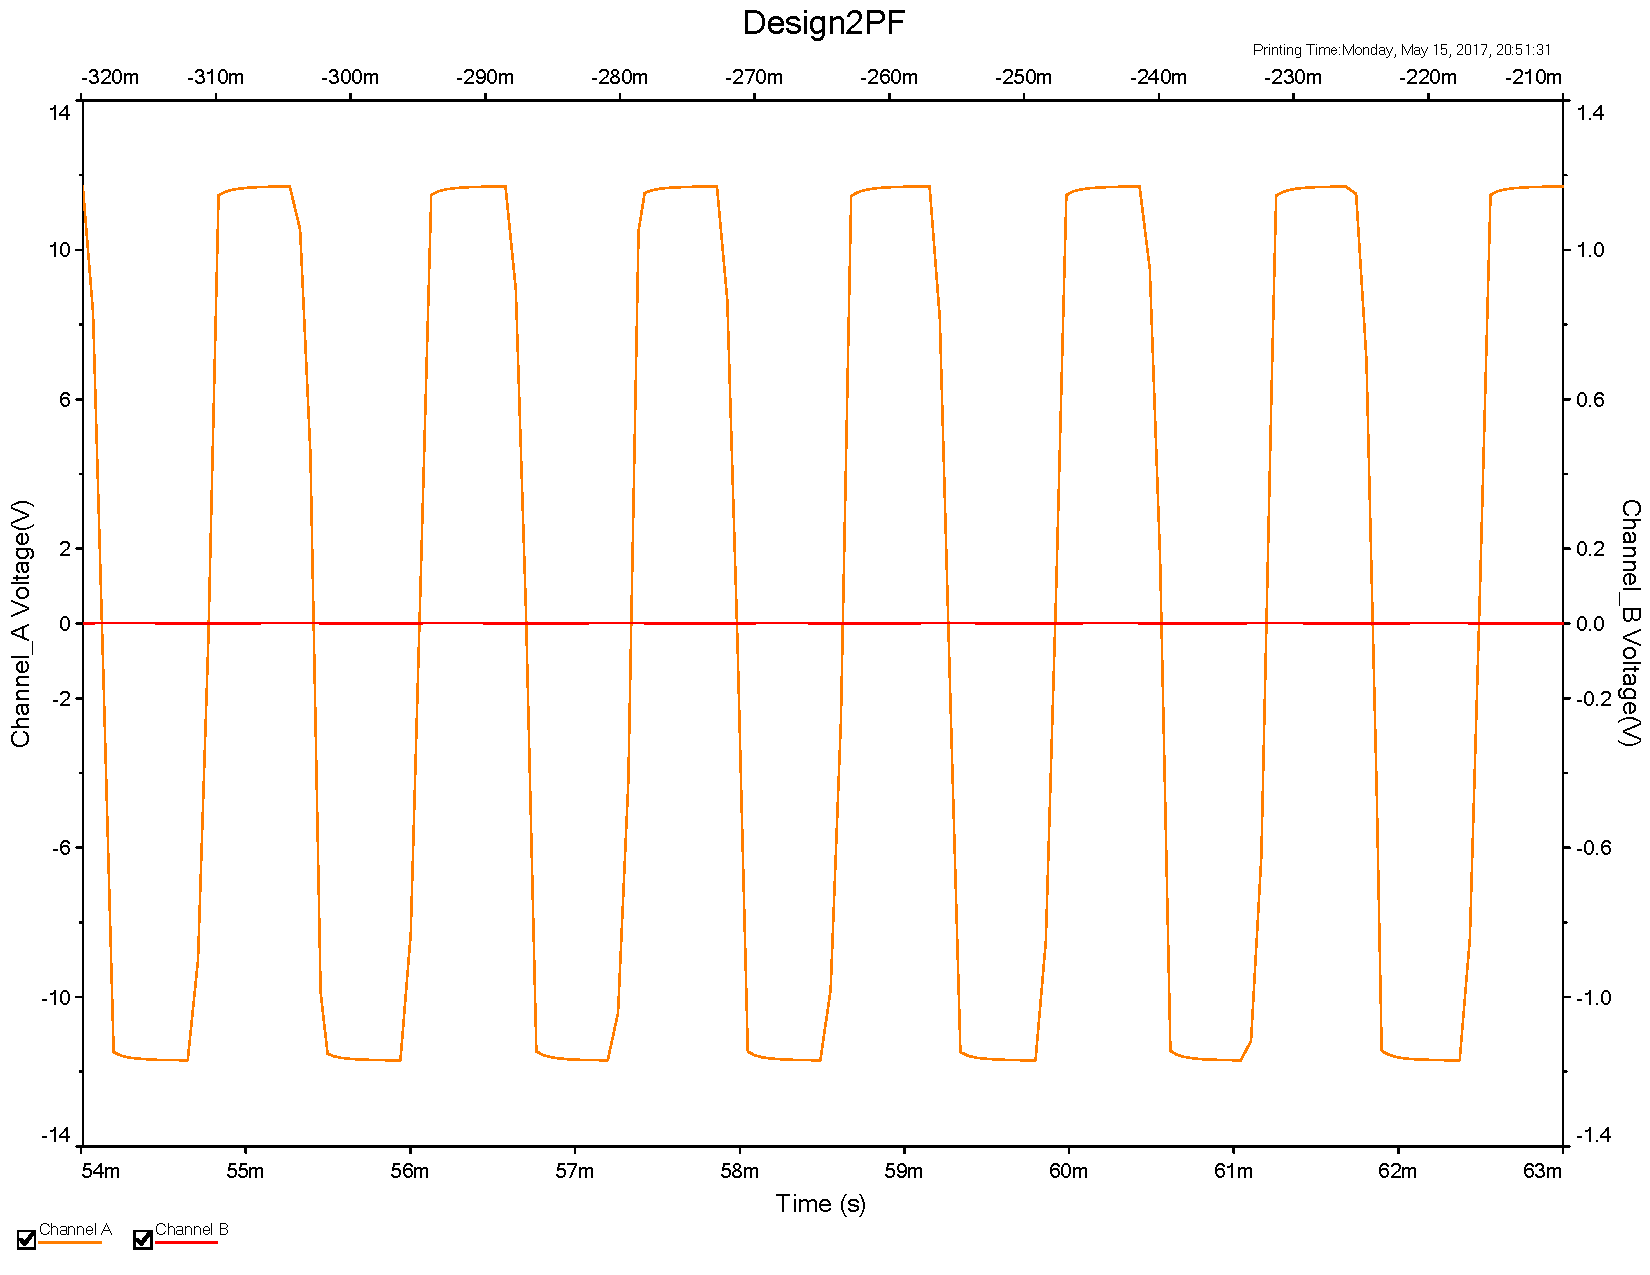
\includegraphics[width=\columnwidth]{2PF.pdf}
\caption{带通滤波器不稳定波形}
\label{BIPF}
\end{figure}
\begin{figure}[H]
\centering
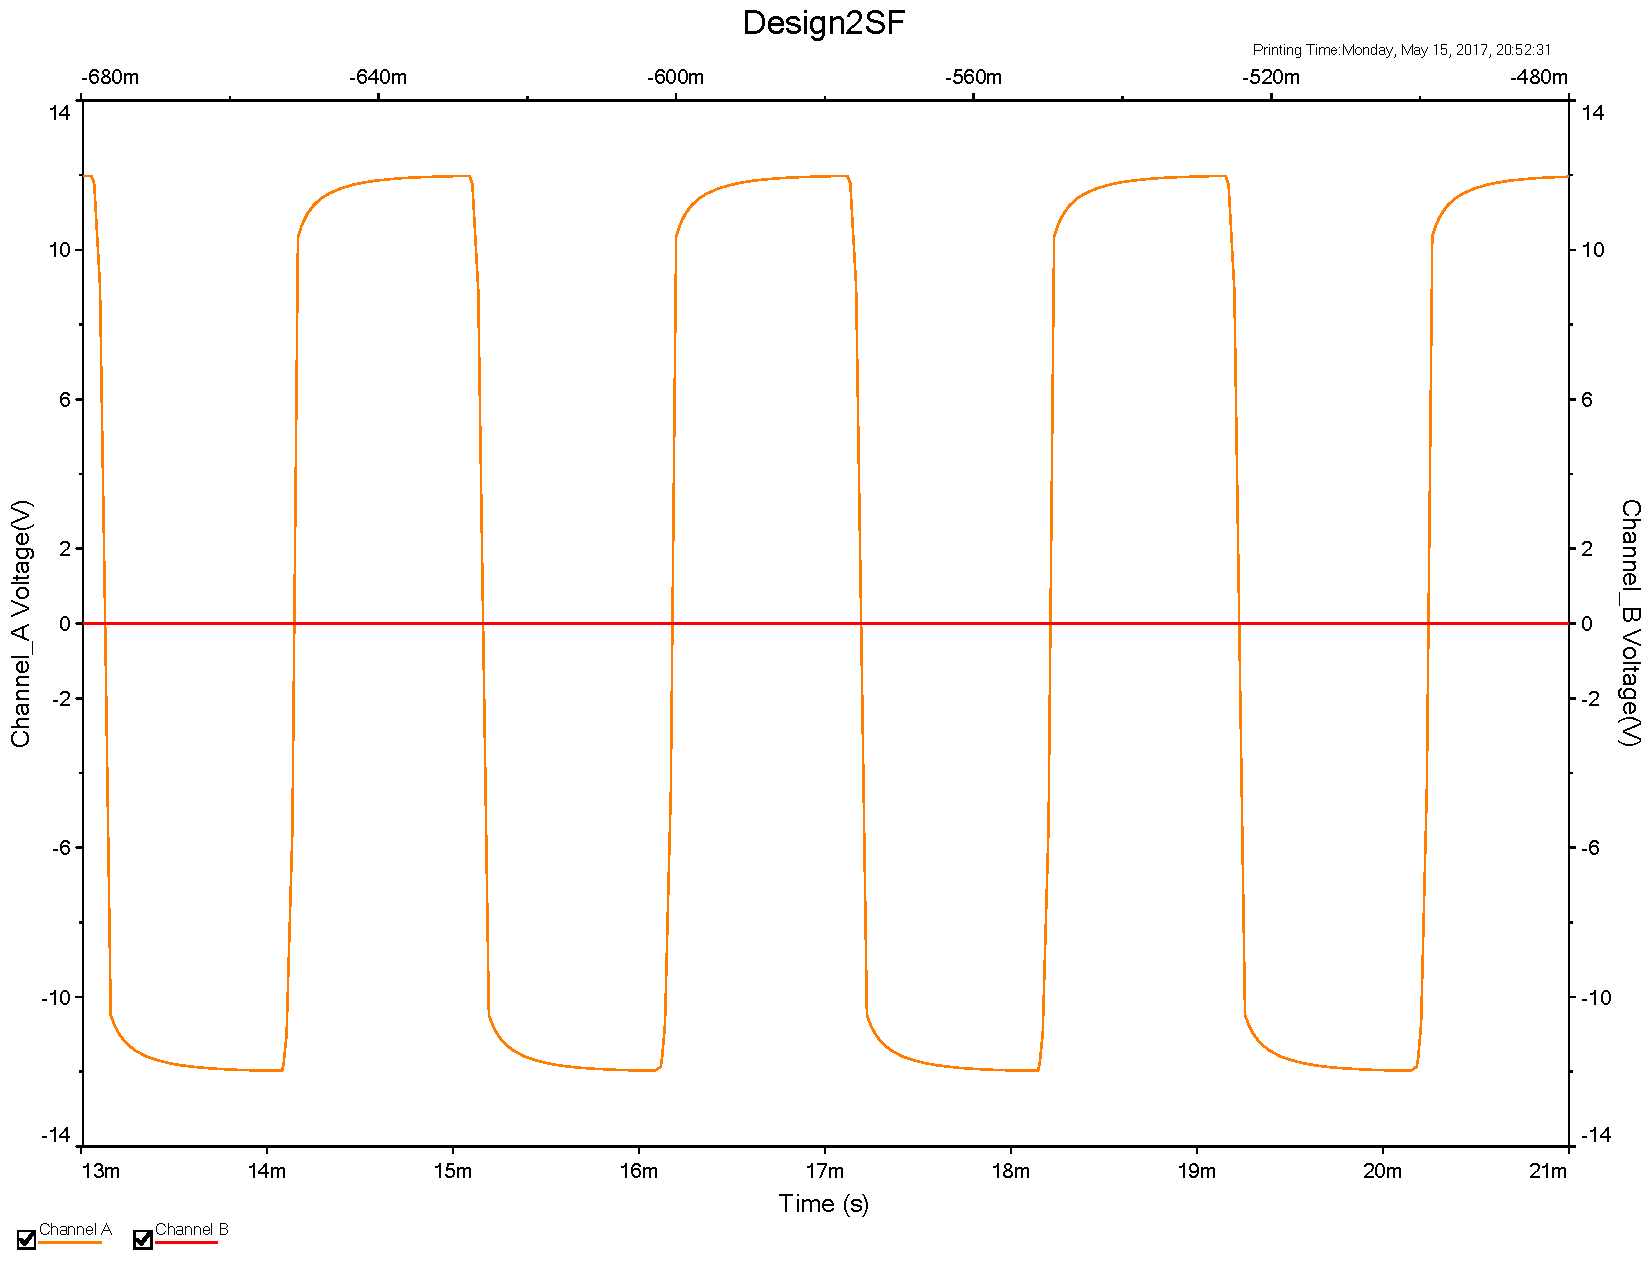
\includegraphics[width=\columnwidth]{2SF.pdf}
\caption{带阻滤波器不稳定波形}
\label{BISF}
\end{figure}
\end{multicols}
\section{波形变换电路(习题7.29)}
设计要求将100Hz正弦波转化为200Hz的锯齿波,如图\ref{cir3}设计了电路
\begin{figure}[h]
\centering
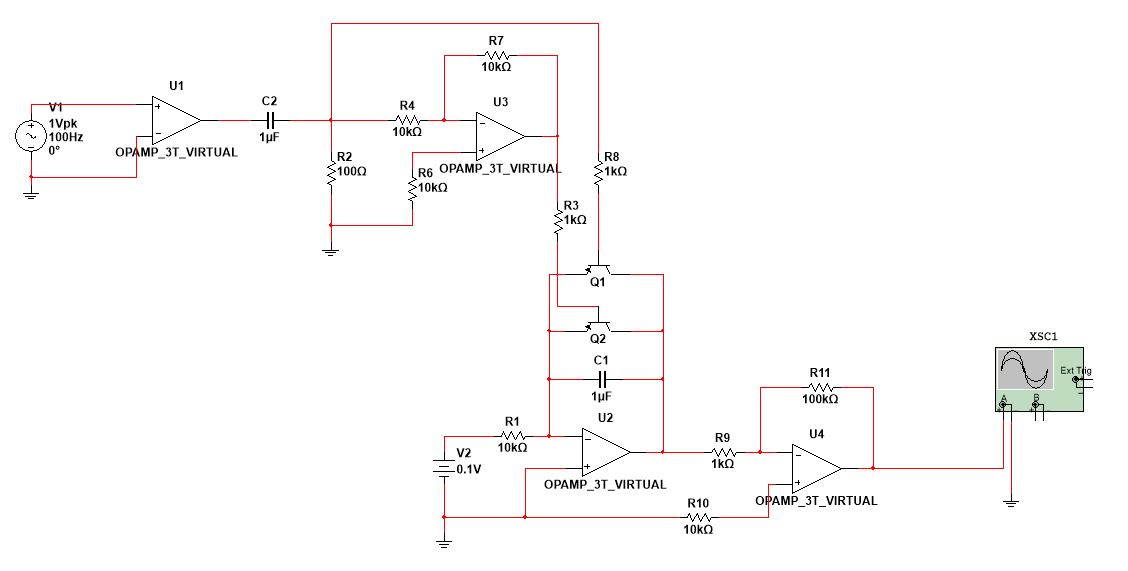
\includegraphics[width=\columnwidth]{cir3.jpg}
\caption{波形变换电路}
\label{cir3}
\end{figure}
首先观察电路可以看出,运算放大器U1是一个过零比较器,U2是一个简单的反相积分器,U3是一个反相器,U4是一个反相比例放大器。

显然,100Hz正弦波经过U1得到一个性能比较好的100Hz方波,假设当前状态下U1输出为正摆幅,电路稳定工作,则$R_2$上的分压为0,电压全部加在$C_2$上,先正弦波过零,电路翻转,输出方波出现边沿变为负摆幅,由于$C_2$上分压瞬时不变,因此$R_2$上出现负偏压。PNP型管$Q_1$射级电压为0,基级电压为负,收到积分过程影响集电极电压为负,因此$Q_1$导通,积分电容开始放电,并几乎瞬间完成。

同样道理,在U1输出翻转到负摆幅的边沿时,$R_2$上出现正压降,经过$U_3$反相之后控制$Q_2$开启来给积分电容放电。

\begin{figure}[H]
\centering
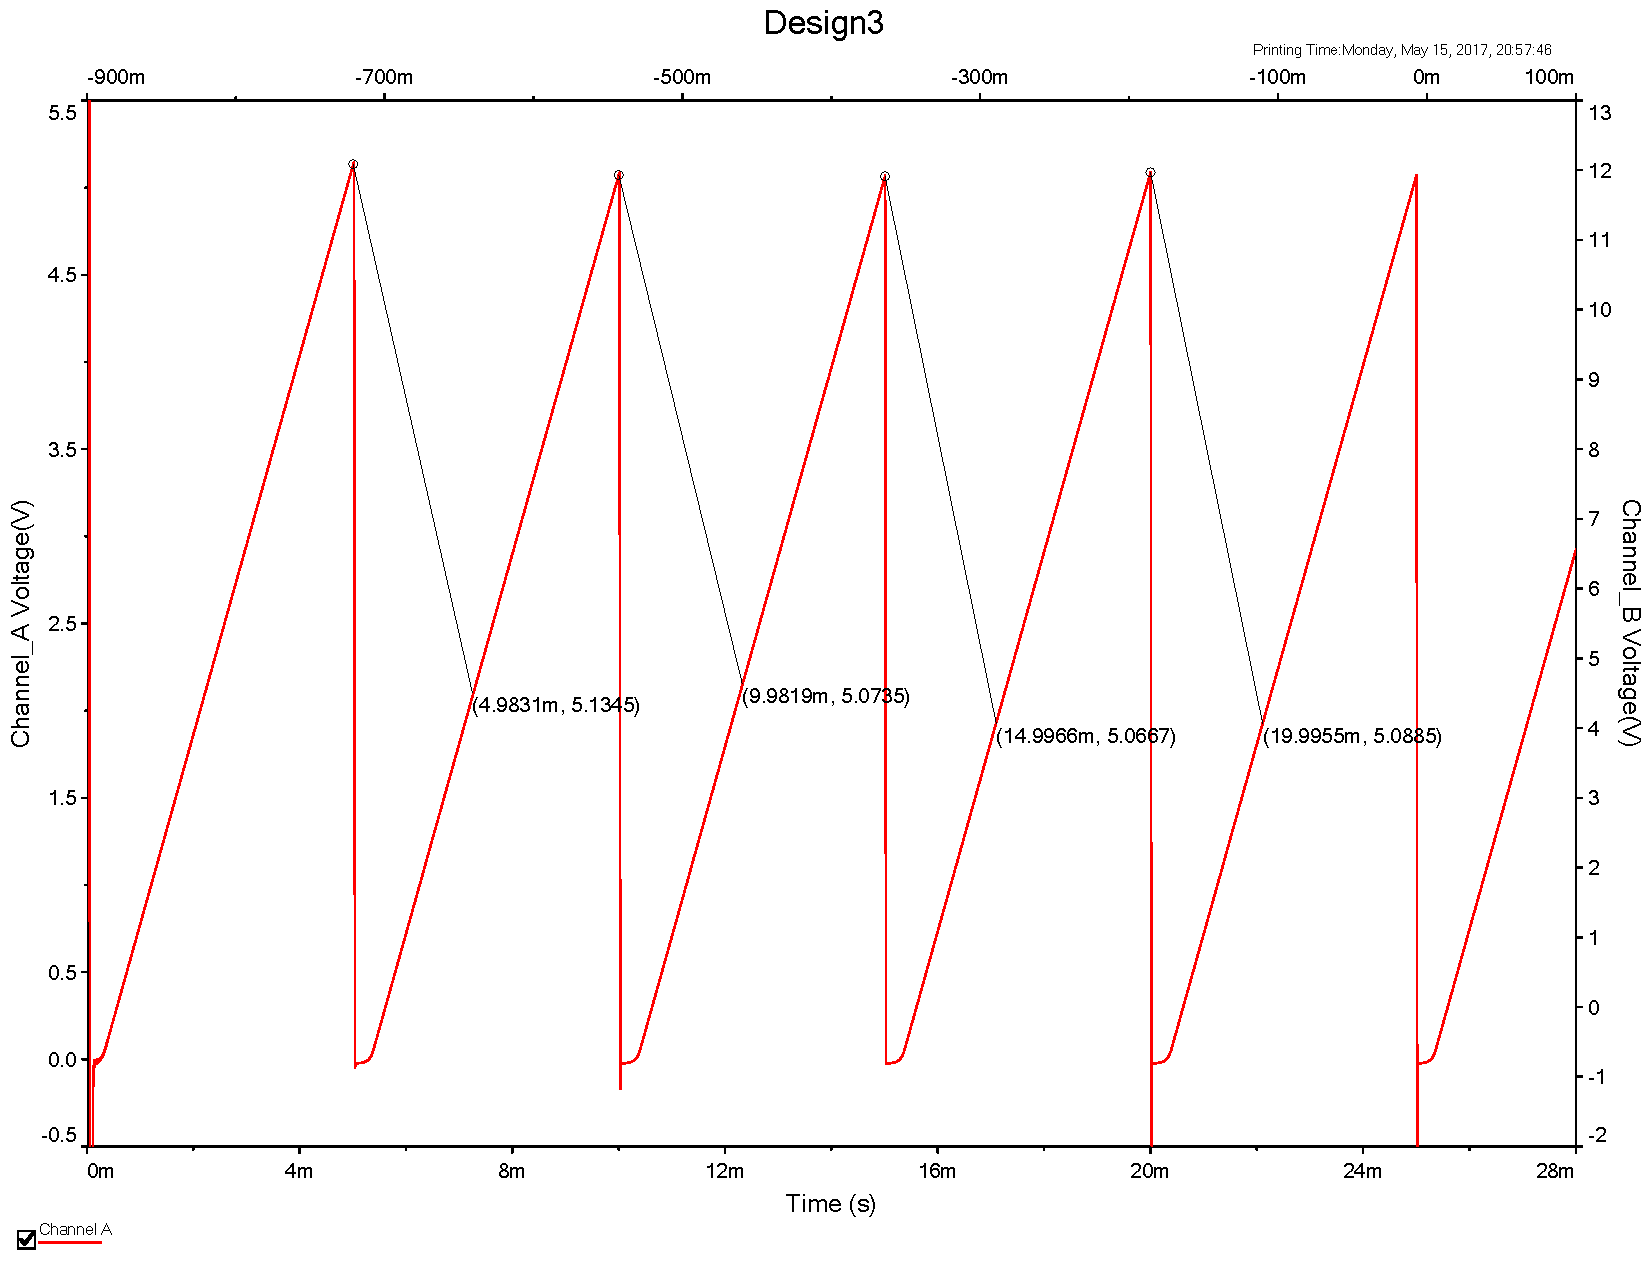
\includegraphics[width=\columnwidth]{wave3.pdf}
\caption{输出波形}
\label{wave3}
\end{figure}

在设计中,考虑到希望放电过程尽可能快的结束,因此不希望U2上积分电容电压过大,因此采用了0.1V直流电压,可以直接看出在不受到$Q_1Q_2$影响时U2的输出为
$$U_{2O}=-10t\mathrm{V/s}$$
经比例放大得到
$$U_O=U_{3O}=t\mathrm{V/ms}$$
同时受到200Hz(U1输出方波两个边沿控制)的放电频率下形成锯齿波,放电间隔为5ms,因此可以得到锯齿波的振幅为5V。

因此如图\ref{wave3}所示得到输出波形,看到输出了一个0到5V的状态良好的锯齿波,锯齿波的下降时间可以忽略不计。幅值基本在5V左右。

\appendixpage
整个仿真工作量较大,为了方便调试和报告的撰写等,将整个仿真分成了若干个Multisim14工程,这里列举如下
\begin{multicols}{2}
\begin{itemize}
\item Design1: 第一题电路 
\item Design2H: 高通滤波器输入方波 
\item Design2H1: 高通滤波器$Q=1$ 
\item Design2H2: 高通滤波器$Q=\frac{2}{3}$ 
\item Design2H3: 高通滤波器$Q=10.5$ 
\item Design2HF: 高通滤波器不稳定设计
\item Design2L: 低通滤波器输入方波 
\item Design2L1: 低通滤波器$Q=1$ 
\item Design2L2: 低通滤波器$Q=\frac{2}{3}$ 
\item Design2L3: 低通滤波器$Q=10.5$ 
\item Design2LF: 低通滤波器不稳定设计
\item Design2P: 带通滤波器输入方波 
\item Design2P1: 带通滤波器$Q=1$ 
\item Design2P2: 带通滤波器$Q=\frac{2}{3}$ 
\item Design2P3: 带通滤波器$Q=10.5$ 
\item Design2P4: 带通滤波器$Q=\infty$ 
\item Design2PF: 带通滤波器不稳定设计
\item Design2S: 带阻滤波器输入方波 
\item Design2S4: 带阻滤波器一种$Q=\infty$ 
\item Design2SF: 带阻滤波器不稳定设计
\item Design3:第三题电路 
\end{itemize}
\end{multicols}
\end{document}